
\documentclass[12pt]{article}
\usepackage[letterpaper, portrait, margin=1in]{geometry}
\usepackage{graphicx} % Required for inserting images
\usepackage{indentfirst}
\usepackage{setspace}
\usepackage{booktabs}
\usepackage{siunitx}
\usepackage{longtable}
\usepackage{amsmath}
\usepackage{authblk}
\usepackage{makecell}
\usepackage{natbib}
\usepackage{float}
\usepackage{xr}
\usepackage{pdflscape}
\usepackage{longtable}
\usepackage{caption}
\usepackage{hyperref}
\hypersetup{
    colorlinks=true,
    linkcolor=blue,
    filecolor=magenta,      
    urlcolor=cyan,
    pdftitle={Overleaf Example},
    pdfpagemode=FullScreen,
    }

\urlstyle{same}
\usepackage{subcaption}
\usepackage{fancyhdr}
\pagestyle{fancy}
\fancyhf{} % clear existing header/footer entries
% Place Page X of Y on the right-hand
% side of the footer
\fancyfoot[R]{\thepage} 
\usepackage{titlesec}
\newcolumntype{d}{S[input-symbols = ()]}
\newcommand{\tabnotes}[2]{\bottomrule \multicolumn{#1}{@{}p{0.70\linewidth}@{}}{\footnotesize #2 }\end{tabular}\end{table}}
\usepackage[flushleft]{threeparttable}
\bibliographystyle{apalike}
%\usepackage{draftwatermark}
%\SetWatermarkText{DRAFT}
%\SetWatermarkScale{5}




\title{The Impact of Natural Disasters on Rents: \\ Evidence from Hurricane Sandy}
\author[]{Katharine WH Harwood}
\affil[]{New York University Wagner School of Public Service}
\date{\today{}}



\begin{document}

\maketitle
\begin{center}
PRELIMINARY DO NOT CITE
\href{}{Click here} for the most updated version of the paper
\end{center}
%TC:ignore
\begin{abstract}
    \small
    This paper explores the impact of natural disasters on rental markets and the role of existing government rental subsidies through the Housing Choice Voucher program in the wake of such destructive events. Combining a novel data set of asking rents in New York City with spatial data on the storm surge flooding incurred by Hurricane Sandy, I estimate the local impact of the storm on affected neighborhoods using a difference in differences design.  In contrast to the literature on home prices after Hurricane Sandy, I find initial negative impacts on rents rebound quite quickly. Evidence of no additional significant change in quality-adjusted rents masks heterogeneity by neighborhood income. Asking rents in above median income neighborhoods increased by roughly 5\% on high surge blocks compared to no surge blocks, while asking rents in below median income neighborhoods were negatively impacted by roughly 5\%. Households and landlords in the Housing Choice Voucher program were largely protected from these market fluctuations. Voucher rents were "sticky" downward, and actually increased by over 5\%, benefiting landlords. Programmatic features allowed for the incidence of these increases to fall nearly entirely on the government, protecting the tenants. These results underscore the importance of examining the impact of disasters on rental markets both for questions surrounding the equity distribution of disaster recovery and for the implicit incentives created by existing rental subsidies to house vulnerable populations in high risk areas. 
\end{abstract}

\vspace{3cm}
\small

\newpage
\section*{Introduction}
\doublespacing
As natural disasters grow in frequency and intensity under climate change, understanding how these extreme events affect housing availability and affordability is increasingly important.   Most studies examining the impacts of hurricanes on the housing market focus on impacts on property values and have generally found that such storms decrease property prices in the affected areas (\cite{bin_changes_2013}; \cite{bin_effects_2004}; \cite{hallstrom_market_2005}; \cite{ortega_rising_2018}; \cite{yi_housing_2020}). Given that rental data is difficult to obtain, few papers (\cite{an_rental_2020}) have been able to focus on rents and theoretically, the impacts of storms on rents might differ from home prices.  For instance, there is less reason to think that storms will reduce rents since renters don’t have the same long-term stake in the property as owners. In fact, supply adjustments may predict rising rents as landlords may be more apt to remove rental units from supply or make investments in repairs that raise properties to the next price tier.  In addition, if the hurricane damage prompted new development, units in new buildings may rent at higher levels.

Examining the role of rental subsidies in the aftermath of a hurricane can shed light on how, due to the nature of the subsidy, this market of renters can experience different impacts of such shocks.  While there is ample evidence showing that low-income and minority neighborhoods are typically more vulnerable to the harmful impacts of such events (\cite{cutter_social_2012}; \cite{van_zandt_mapping_2012}), low-income households may also be shielded from market fluctuations by subsidies they receive. Landlords may be able (required) to renovate their properties earlier than other low-income landlords, and programmatic features may allow them to recoup renovation costs through rents without risk of losing their tenants.  This effective "insurance" spurs questions surrounding the incentives created to house at-risk populations in neighborhoods especially susceptible to such damage. Rents may not be bound to the market forces in the rest of the low-rent market. To understand the ways in which government intervention is altering impacts for those it supports, examining the population of existing rental subsidy recipients is critical.

In this paper, I first examine the localized effect of Hurricane Sandy on rental markets in the affected neighborhoods and examine several dimensions of heterogeneity in the impacts. I then turn to questions surrounding the role of government rental subsidies through the Housing Choice Voucher program in affecting the rental impacts for low income households. Hurricane Sandy (2012) is an ideal storm to study these questions because it was a large, and sudden event that caused substantial damage across the city, but the storm surge affected the city in somewhat unpredictable ways. This meant that neighboring blocks experienced wide variation in damage from the storm, providing plausibly quasi-exogenous variation across otherwise similar, small geographic areas. 

Exploiting this variation, this paper is able to make two main contributions to the existing literature on housing markets in the wake of disasters. First, by combining a new and unique data set of unit-level asking rents from StreetEasy listings with spatially detailed information on storm surge heights and flood zones, I am able to assess the impacts of the storm on market rents by comparing smaller geographic areas than other papers on rental impacts (\cite{an_rental_2020}).  Using an event study methodology, I find that, immediately after the hurricane, rents in affected areas decreased relative to non-affected areas within in the same zip code by 5 percent.   This drop likely reflects a dis-amenity effect from the blight and damage incurred, further supported by the fact that no such drop occurred in low surge areas. It is also consistent with the work of Meltzer et al. (\citeyear{meltzer_localized_2021}), which found that retail businesses on blocks with high storm surge levels experienced a change in closure rate that was twice as high as that for establishments in areas without any surge. The effects were also particularly pronounced in the years immediately following the storm.    

However, in contrast to the literature on home prices that shows persistent 11-22\% price discounts for at least 6 years after Hurricane Sandy (\cite{ellen_heterogeneity_2022}, \cite{ortega_rising_2018}), rents rebounded quite quickly.  Two years later (by 2014), quality-adjusted asking rents in high surge areas had recovered substantially and by four years post-storm they had returned to rent levels in non-surge areas. 

Yet the average impacts mask heterogeneity in response by neighborhood income.  Quality-adjusted rents in above median income neighborhoods increased by roughly 5\% more on high surge blocks than no surge blocks after the hurricane, while quality-adjusted rents for below median rent units decreased by roughly 5\%.  These differential impacts are consistent with some literature that finds that higher income households are more likely to stay in their units in the wake of a disaster and invest in protection against future storms rather than move (\cite{smith_adjusting_2006}).  Residents of these neighborhoods have more resources, and they appear to have renovated their properties more quickly. Ellen et al. (\citeyear{ellen_heterogeneity_2022} find that above median income neighborhood home prices recovered more quickly than below median income neighborhoods. These impacts could also reflect less initial blight, and therefore no corresponding drop in demand, in higher income neighborhoods. 



%  In addition, average (non quality-adjusted) neighborhood rents had increased by nearly 3.6\% on high surge blocks compared to non-surge blocks within the same zip code by 2014, and by 2019 this differential had increased to nearly 5 percent.  Off a baseline average of about \$4,387 a month, these differences represent roughly \$158 and \$219 respectively. 

% I find evidence of a shift in the composition of the rental stock toward more new, high-rent buildings. After the hurricane, there was a spike in both demolition and new construction in high surge areas. Newer buildings generally rent at higher levels than older buildings since they are often of higher quality with newer amenities, so an increase in new buildings replacing older buildings could push up average neighborhood rents.  In addition, the buildings built in high surge areas after the hurricane had higher rents than their counter parts in non-surge areas.


% The higher rents could also could also reflect increased demand for newer buildings, driven by the information shock of the storm.  Many papers on the impact of information from storms having taken advantage of the flood zone boundary to isolate the information effects (\cite{meltzer_localized_2021}; \cite{ellen_heterogeneity_2022}; \cite{hallstrom_market_2005}; \cite{gillespie_information_2020}).  The assumption in these analyses is that households within the flood zone would have had more information about the riskiness of their neighborhoods prior to the hurricane than those outside the flood zone, so the difference between the impacts for those affected by the storm in and outside the flood zone represents the effect of new information.  

% Consistent with these papers, the results here are strongest for affected areas outside of the 100-year flood zone.  This may reflect that renters are updating their beliefs about the riskiness of these neighborhoods and preferring to live in newer buildings they may perceive as less susceptible to flooding, though buildings outside of the flood zone were not required to comply with updated flood-resistant construction requirements (\cite{nyc_building_code_new_2008}, \cite{nyc_department_of_buildings_rebuilding_2015}.  

The second contribution of this paper, is to examine the sub-market of households receiving Housing Choice Voucher subsidies in affected areas, to understand how their rental impacts may have differed from those in other low-income neighborhoods.  While there is considerable literature documenting the distortions created by explicit subsidization of disaster relief through insurance (\cite{kousky_learning_2010}; \cite{gregory_impact_2017}; \cite{gallagher_learning_2014}) and a burgeoning literature on the implicit subsidization of development and habitation of areas prone to damage from climate change (\cite{ostriker_effects_2022}; \cite{baylis_moral_2019}; \cite{wagner_adaptation_2022}), little work has examined the role of existing, non-disaster specific subsidy programs in distorting impacts after disasters. The nature of the subsidy distributed through the Housing Choice Voucher program, and the government's explicit desire to keep these vulnerable populations housed, provide reason to think that rents in this sub-market may behave differently than the low end of the rental market over all. Given the increasing frequency of climate-related disasters and the enormous scale of the devastation they inflict, the question of the degree to which existing subsidy programs alter disaster-related rental impacts for these households is crucial. 

In the Housing Choice Voucher program, the local housing authority pays the difference between the rent charged and 30 percent of a tenant’s income, up to the rent ceiling.  Therefore, as long as the rents landlords charge to voucher holders remain below the allowable rent ceilings (payment standards), rent increases will be paid for by the housing authority\footnote{When households first enter contract on a new apartment with a voucher subsidy, the program requires that the tenant pay no more than 40\% of their income to rent, but no such official limitation exists as the voucher holder remains in the unit.}.  Voucher rental impacts might differ from those in other low-income neighborhoods in two important ways.  First, voucher rents might be "sticky" downward for sitting voucher units. Local housing authorities conduct rent reasonableness assessments when new tenants lease a unit, and when a landlord requests a rent change.  Since it is unlikely landlords would request a rent decrease in line with other units in the neighborhood, they may have been protected from the negative impacts experienced by other units in low-income neighborhoods.   Second, voucher landlords might be able to avoid liquidity constraints on making repairs that other low-income landlords experience if the housing authority acknowledges improvements to their units through rent increases not incurred by the tenants themselves.  They may have been able to, or required to, make repairs to their units earlier, knowing that they could recoup the costs through rent increases without the risk of losing their tenant.  This could have been possible if housing authorities adjusted payment standards to prevent additional rent burden on the tenants, or if original rents were below the payment standards to begin with.  Housing authorities may have prioritized keeping tenants in their units at a vulnerable and chaotic time, over disagreements with landlords over rent hikes.  

I analyze the change in rents charged to voucher holders with the same event study methodology using administrative records from HUD’s housing choice voucher program, and, in contrast to the broader findings, I find a steady relative increase in voucher rents in high surge areas compared to non-surge areas.  Voucher rents appear to have been "sticky" downward: within three years (by 2015), voucher rents had increased by 3 percent (\$45) in high surge areas relative to non-surge areas and by 2017 they had increased by 5.2\% percent (\$87) more in high surge areas than no surge areas. I also find differential increases in rents in low surge areas compared to non-surge areas, which, though noisy, appear to be of similar magnitude to the changes in high surge areas. These rent increases are driven by voucher buildings that filed for renovation in the year immediately after the storm (2013). Voucher landlords were nearly 10\% more likely to file for renovation permits in 2013 than other low-income neighborhoods. This suggests that, in contrast to other units in high flooding, low-income neighborhoods, voucher landlords improved the quality of their units quickly, and rents subsequently increased.  Therefore, voucher landlords appear to have benefited from the distortions created by the housing subsidy.

It appears landlords were able to capitalize quality improvements into rents so quickly because voucher tenants were shielded from the rent increases by the housing authority. I find that the incidence of these Sandy-induced rent increases for subsidized households fell nearly entirely on the government.  There was virtually no increase in the portion of rent paid by voucher holders in high surge areas compared to no-surge areas in the same ZIP code, and the payments from the housing authority mirror the increases in the contract rents.  This may reflect a willingness on the part of the housing authority to accommodate voucher landlords' renovation of damaged properties while keeping voucher holders in their units. 

Together, the results in this paper imply that when considering the impacts of climate change on the housing market, we should consider both the home sales and rental markets, as the impacts may differ between the two. In the case of Hurricane Sandy, while considerable research suggests the hurricane lead to a persistent decrease in home sales prices, I find evidence that while hedonic rents decreased initially, they rebounded much more quickly than home sales prices.  Average effects on quality-adjusted rents can mask considerable heterogeneity in disaster recovery across neighborhood income. 

%In addition, the composition of the rental stock in affected areas changed, which may have longer term implications for neighborhood rents and residents. 
 
The fact that the nature of the subsidy created different rental impacts in the Housing Choice Voucher sub-market should also prompt discussion about the role of existing rental subsidies in the wake of natural disasters.  The housing voucher program appears to have shielded both landlords and tenants from broader market fluctuations by shouldering additional costs. This additional level of "insurance" afforded to landlords might encourage participation in a program plagued by low landlord engagement. However, it may also mean that rental subsidies create an implicit incentive for housing vulnerable populations in neighborhoods at high risk of disaster-induced damage.

This paper is organized into two sections.  Section A focuses on documenting the impact of the storm on asking rents, and details theory and background, data and empirical strategy, results and mechanisms related to this question.  Section B turns to the government's role in insuring low income tenants and their landlords against the rental impacts of climate change, and describes the background and data on the Housing Choice Voucher program, a few small modifications on the empirical strategy, and the results and mechanisms for this question. I then discuss some robustness checks pertaining to both sections.  Finally, the paper concludes with a discussion of the two sections and the policy implications. 

\section*{A. The Impact of Hurricane Sandy on Market Rents}
\section{Theory and Background}{\label{sec:Theory}

Although considerable work has has focused on the impacts of natural disasters on house prices, the theoretical impacts on rents are ambiguous. On the one hand, rents may decrease if demand for rental housing in these areas decreases due to blight or information shocks.  However, rents may increase if there is a substantial reduction in the rental supply, or changes in the composition of the rental stock due to rebuilding or renovations.  A priori, it is not clear which effects should dominate. 

\subsection{Hurricane Sandy}{\label{sec:sandy}
 Hurricane Sandy hit the east coast of the US in October of 2012 and provides an ideal setting for studying the impact of natural disasters on rental markets for two reasons.  First, the hurricane caused considerable damage across a fairly large geographic area.  In New York City, it inflicted roughly \$19 billion in damages and damaged over 69,000 residential properties.  The storm surge affected nearly 9 percent of residential units in the city (NYC.gov).  

  To distinguish areas that experienced higher levels of damage from lower levels of damage, I follow previous work of \cite{ellen_heterogeneity_2022} and designate areas as high surge if they experienced more than 2ft of surge and low surge if they experienced 0-2ft of surge\footnote{This categorization is discussed in more depth in both Sections \ref{sec:Data} and \ref{sec:Estimation}.}.  Figure \ref{fig:zipmap} shows a map of zip codes across the city, with blocks shaded by this storm surge designation. Naturally, most of the high surge areas are along the coast, though notably many blocks along the coast line experienced low or no surge. The surge also covered all five boroughs of New York, generating substantial variation in the populations and neighborhoods affected.
  
  Second, the storm surge was somewhat unpredictable and varied substantially, creating exogenous variation in storm exposure across neighboring city blocks. Figure \ref{fig:ues} provides an example of an Upper East Side neighborhood where the surge levels vary considerably across neighboring blocks, as well as across the flood zone boundary, depicted in grey.  High, low, and no surge blocks are contiguous and cross in and out of the flood zone, creating plausibly exogenous "treatment" and "comparison" groups across small geographic areas.

\subsection{Potential Rental Effects of Storms on Housing Markets}{\label{sec:markets}

\subsubsection*{Reduction in Rents}
Damage from a hurricane make affected neighborhoods less desirable, either because of the blight incurred or because of new information about the riskiness of the neighborhood.  Research has shown evidence of such a negative demand shock in the homeownership market.  Several papers document negative effects of hurricane and flooding risk on residential property prices (\citep{bin_effects_2004}; \cite{ortega_rising_2018}; \cite{gillespie_information_2020}; \cite{hennighausen_flood_2020}).   Many of these papers also find that new information about the relative riskiness of neighborhoods is a strong driver of the decrease in demand in the longer term. Hallstrom and Smith (\citeyear{hallstrom_market_2005}) find that prices decreased in counties that did not experience damage from Hurricane Andrew, but where the hurricane would have conveyed risk information to the homeowners. Ellen and Meltzer (\citeyear{ellen_heterogeneity_2022}) find evidence that after Hurricane Sandy, while housing prices decreased in areas affected by the storm across the board, prices remained depressed for a longer period of time outside the flood zone than inside the flood zone.  They suggest that prospective buyers of properties outside the flood zone received new information about the relative riskiness of the properties that was already known to buyers within the flood zone through the requirement to purchase flood insurance and that this outweighed any existing supply effect. Kousky (\citeyear{kousky_learning_2010}) shows a similar effect in Missouri, where property prices in 100-year floodplains did not change significantly after a 1993 flood of the Mississippi River, but prices in the 500-year floodplains significantly declined where home buyers would not have initially been informed about their property's flood risk.

It is not clear, however, how strong we should expect the negative demand effect to be for renters.  Renters experience the same dis-amenity effect of blight as homeowners, but renters do not have the same long-term stake in property as owners. Renters care  about the use-value of housing, and are not concerned with the long term asset value of the unit.  In addition, they are not required to purchase flood insurance and are less likely to need to pay for repairs if damages are incurred.  Flood zone and surge level boundaries are likely to be less salient borders to renters and renters have less reason to be discouraged by potential long-term outcomes of property in these areas. 

That said, renters may have less initial information about flood risk than homeowners since they are not required to purchase flood insurance, and thus storms may provide a larger information shock to renters.  While they are not likely to incur large repair costs to the unit, they may suffer damage to personal property.  In addition, if enough displaced households join the rental market in the short-run, rental demand could increase. However, it's not clear where we would expect displaced households to choose to rent, and therefore what the impact would be on rents in damaged areas.  If they choose to rent very near to their damaged home, this increased in rental demand might drive up rents.  However, if they choose to rent on non-damaged blocks, given the experience they just incurred with their home, we might actually see rental increases in unaffected areas relative to highly affected areas. 

\subsubsection*{Increase in Rents}
Other mechanisms might lead to an increase in rents. The damage inflicted by the storm might initially considerably reduce the supply of rental housing, with fewer habitable properties leading to a rise in rents for the remaining stock (\cite{vigdor_economic_2008}).  In the case of Hurricane Sandy, which damaged but did not completely destroy many properties, the supply of viable rentals in surge areas could arguably be more elastic than the supply of owner-occupied homes.  It may be too costly for smaller landlords to maintain rental units in at-risk areas.  These landlords may remove their damaged units from the market entirely, particularly in the case of basement apartments, while continuing to occupy higher floors of their buildings. This could lead to a considerably larger reduction in the supply of rental units than owner-occupied properties. 

In addition, other factors may alter the composition of the rental stock.  Damages may lead landlords to renovate or rebuild their properties, potentially improving quality and pushing their units into the next tier of the rental market. New development to replace damaged properties might lead to newer units driving up rents. It's also possible that older, damaged buildings were removed from the rental stock altogether, creating a younger rental supply in affected areas, which is strongly correlated with higher rents.

At the intensive margin, ownership may play a role.   It's possible that, if landlords are constrained by their ability to recoup renovation costs, they choose to sell their buildings after the hurricane. This may be particularly true for smaller landlords who may have more liquidity constraints.  Heightened turnover may bring in a set of new owners with different business models, which may lead to a change in rents.   Even if the volume of sales is unchanged, it’s possible that buyers who are willing to take on the risk of a rental property in an area susceptible to damage may be larger, and more resourced.  These buyers may be more sophisticated in their knowledge of the market and more aggressive in increasing rents to the maximum the market can bear. Even if ownership does not change, reactions to the hurricane may vary by landlord type. Indeed a working paper by Verbugge and Gallin (\citeyear{verbrugge_theory_2017}) suggests that rents are stickier for small landlords than for larger landlords, who are less affected by the costs incurred from losing a tenant. 

\subsubsection{Heterogeneity by Submarket}
Finally, the overall impacts on rents in affected areas might mask important heterogeneity across several dimensions.  Several papers have explored the impacts of disasters on home prices stratified by neighborhood income, with mixed results. Smith et al. (\citeyear{smith_adjusting_2006}) find that higher income households are more likely to stay in their homes and invest in preventing further damage, while lower income households prefer to move to more affordable housing. Cohen et al. (\citeyear{cohen_storm_2021} and Ellen et al.(\citeyear{ellen_heterogeneity_2022}) actually find larger initial impacts in higher income neighborhoods, but the latter find that these neighborhoods recover more quickly.  They suggest their results may reflect that residents of higher income neighborhoods may have more resources to repair damage and blight, and to ensure themselves from damage from future disasters.  On the other hand, higher income renters are likely to be much more mobile than lower income renters, so we might expect a larger response in demand in higher income areas.

We might also expect to see heterogeneity along building characteristics, such as height, renovations and landlord turnover.

Ultimately, since the theory suggests the possibility of a variety of countervailing forces, the question of the impact of the hurricane on rents in affected neighborhoods is an empirical one. 

\section{Empirical Strategy} 

I estimate the impact of Hurricane Sandy on rents using a difference-in-differences design that compares blocks that experienced higher levels of storm surge to blocks that experienced no storm surge within the same zip code. To do this, I gather a rich data set of spatially detailed data on the storm surge from the hurricane, market rents and administrative data from New York City.

\subsection{Data}{\label{sec:Data}

\subsubsection*{FEMA Surge and Flood Maps} 
I use FEMA's surge map to capture the impact of the storm through water inundation.  The FEMA Modeling Task Force (MOTF), a group that uses statistical modeling and on the ground surge sensors and field observations to regularly update flood impacts, uses high-water marks and surge sensor data to interpolate water surface elevation after the storm.  They report surge levels at one or three square meters but following previous work, I collapse these interpolated micro estimates to the block level (\cite{ellen_heterogeneity_2022}).  

I categorize surge heights to facilitate a comparison between areas that were clearly impacted by the storm and those that were not. In Figure \ref{fig:scatdam}, I examine the relationship between surge heights and FEMA's estimate of "major damage"\footnote{I choose to use surge heights rather than FEMA's plot level estimates of damage because surge heights are a major factor that goes into FEMA's damage calculation and surge heights are more likely to be exogenous to rental changes than damage.  This follows other papers on Hurricane Sandy (\cite{ellen_heterogeneity_2022} and \cite{meltzer_localized_2021}).}, aggregated to the block level, to find an appropriate surge-level threshold to identify blocks that were severely affected by the storm.  The main goal of identifying a surge-level cut off is to capture as many blocks that experienced major damage due to the storm as possible, while excluding properties that were likely damaged due to other, potentially endogenous, factors, like the quality of the structure.  The red line indicates a block level average of 2ft, this paper's threshold for categorization as a "high surge" block.   Using the 2ft threshold, properties that did not experience any surge but still incurred a substantial amount of damage, and properties that experienced low levels of surge and damage are excluded from being categorized as highly affected by the storm.  While 2 feet appears to be a reasonable threshold, I do experiment with other surge thresholds, as discussed more in section \ref{sec:Estimation}.   

With a 2ft threshold for "high surge" areas, "low surge" areas are designated as experiencing flooding, but with less than 2ft of water and no surge blocks did not experience any storm surge.  I also use the boundaries of the 100-year flood zones in effect at the time of Hurricane Sandy and categorize areas into high-risk areas (flood zone = 1) and low risk areas (flood zone = 0). 

\subsubsection*{Asking Rents} 
To examine the impact of the hurricane on asking rents, I use unit-level asking rent data from 2010-present from StreetEasy, provided through a partnership with the Furman Center. The data includes the asking rent for the unit, the number of bed and bathrooms in the unit, whether the unit listing required a broker fee, the date of the posting, the address and geolocation. 

Since StreetEasy started in 2006, by 2010 it was still relatively nascent.  While at present, StreetEasy is ubiquitous in rental searches in New York City, at the time of Hurricane Sandy StreetEasy listings were concentrated in high rent neighborhoods and buildings.  Figures \ref{fig:seborough} and \ref{fig:sebuild} show the composition of the sample over time across borough and type of building, respectively. Listings are concentrated in Manhattan, especially in the early years, though Brooklyn and, to a lesser extent Queens, gain listings over time period.  Listings are predominantly in elevator buildings, condo buildings or walk-ups or 3 or more units, initially, though the share of listings in walk-ups increases dramatically from 2010-2015.  By the end of the period walk-ups make up a greater share of listings than elevator buildings. 

Figures \ref{fig:2011sesample} and \ref{fig:fullsesample} show the geographic distribution of listings in the sample by surge area, first in 2011, and then across the whole time period.  They reflect the same initial concentration in Manhattan and subsequent spread to other boroughs, across all three surge designations. The same apartments do not appear often enough in the sample to attempt a repeat-rent model, however it is noteworthy that, while the increase in listings is clear over time, most listings are concentrated in ZIP codes that contained listings before the storm.  This means that limiting the sample to ZIP codes that appear in 2010 and 2011 still captures over 90\% of listings in the entire sample.

Overtime, the sample across all three surge areas increases in the number and variety of listings. Plotting the average asking rents over time misleadingly indicates a decrease in rents over the time period as more lower-rent units are added to the sample.  Figure \ref{fig:rentchange} plots the average block level change in rent from the prior year, holding constant the number of bedrooms, over time. It is clear that around the time of the hurricane there is more volatility on high surge blocks than low and no surge blocks, with almost no increase in average rents the year after the hurricane, and then increasing by more than \$200 in 2015 compared to an increase of around \$100  in low and no surge areas.  This volatility is particularly notable given how closely the trends track each other later in the period. However, it is important to note that over much of the time period, with the most dramatic exception in 2020 when COVID first hit, rents were increasing each year across all three surge groups.  As discussed in more detail under Section \ref{sec:Estimation}, the impacts found in this paper are relative to the comparison group and do not reflect absolute changes in rents.


\subsubsection*{Building permits}
To observe whether rent changes are associated with new building permits, demolition permits, or renovation permits for damaged properties, I include Department of Buildings (DOB) data on jobs permits during the time period. This data is collected by the city for all job applications submitted through the Borough offices since January of 2000.  Jobs are classified as “new building”, "demolition" or "alteration". Alterations are further classified as "A1", for "a major alteration that will change the use, egress, or occupancy of the building", "A2" for "an application with multiple types of work that do not affect the use, egress, or occupancy of the building" and "A3" for "one type of minor work that doesn't affect the use, egress, or occupancy of the building."  Of the renovation permits in the sample filed within four years of the storm (2013-2016), 65\% were categorized as "A2", 33\% as "A3" and only 2\% were categorized as "A1".

\subsubsection*{PLUTO} 
To identify characteristics of buildings, I use the city's publicly available Primary Land Use Tax Lot Output (PLUTO) building data from 2007 - 2021.  This data includes annual extensive land use information at the tax lot level.  I match on the tax lot number (BBL) to retrieve the number of units in the buildings, the number of floors, and the age of the building. 

\subsubsection*{Building Sales}
I use data from the Department of Finance (DOF) combined with the Automated City Register Information System (ACRIS) to obtain information on property records and deeds from 2004 -2019.  This data includes the date of sale, as well as the name of the seller and of the buyer.  I use this data to observe the number of sales over time in affected areas, and whether rents change after an arm's length sale occurs. 

\subsection{Summary Statistics}

To identify whether rents changed in neighborhoods impacted by the hurricane, I limit my sample to zip codes that have at least one census block that experienced some level of surge.

Table \ref{tab:marketsamp} reports the number of individual listings, census blocks, and zip codes in the StreetEasy sample in 2011, one year prior to the hurricane, and for 2017. In 2011 there were 2,070 listings in 110 blocks that would experience high levels of surge across 56 different zip codes. As noted previously in section \ref{sec:Data}, in 2011 StreetEasy was a relatively new service in earlier years of the time period so the sample grows over time.  

Table \ref{tab:marketstats} shows baseline (2011) summary statistics for StreetEasy units by surge level.  Units in high surge areas tend to look fairly similar to those in the comparison group, no surge areas, though notably the buildings they are in are about 10 years younger, the neighborhoods are slightly whiter with slightly lower median neighborhood rents.  Low surge units tend to be in substantially larger and newer buildings, with higher baseline average rents. 


\subsection{Estimation}{\label{sec:Estimation}}
I estimate the impact of Hurricane Sandy on rents in the affected neighborhoods using a difference in differences methodology that compares census blocks that experienced high and low levels of surge to census blocks within the same zip code that experienced no surge before and after the hurricane. I begin with following standard difference in differences equation 

\begin{equation}
\label{eq:DID}
\begin{split}
y_{ht}= \sigma_{z(h)}\ast\tau_t+\sigma_{z(h)}\ast surge_{b(h)}  + \sum_{s\in S}{\beta_{t,s}Post_{t}\times \mathbb{1}}(s(b(h))=s) \\+\gamma_{1}floodzone_{h} + \theta X_{ht} + +\varepsilon_{ht}
\end{split}
\end{equation}

Where y is the log rent in \$2021, for housing unit h, in time t.   Within the summation, $Post$, an indicator for years post 2012, is interacted with a set of dummy variables indicating the surge level, s(b(h)) of the block, b, on which the housing unit is located, so the set s is defined as $S = {high, low}$. High surge blocks experienced storm surge levels of more than 2ft of water, and low surge blocks experienced surge levels of less than 2ft. As discussed in Section \ref{sec:Data}, I experiment with other thresholds and find qualitatively similar results, shown in Appendix Table \ref{tab:surgelevs}. 

  Importantly the equation contains zip code by year ($\sigma_{z(h)}\ast\tau_t$) and zip code by surge level fixed effects  ($\sigma_{z(h)}\ast surge_{b(h)}$) to remove variation from time trends in the zip code and baseline differences between surge levels in the zip code.\footnote{Impacts using census tract fixed effects instead of zip code show very similar results. See Figure \ref{fig:tractfe}.}  This allows for the interpretation of the coefficients of interest, $\beta_{t, s}$, to be the changes in rents in high and low surge areas, relative to non surge areas within the same zip code, before and after the hurricane. 
  
   I include a vector of housing unit characteristics, ($X_{ht}$), which include, the number of bedrooms and bathrooms, and whether the unit required a broker fee.  I also include building level controls including the number of units in the building, units squared, the age, age squared and the number of floors, and whether the unit is located in a building with subsidized or controlled rents, where regulations might have prohibited rental increases. 
   
  In addition, I include an indicator for whether the unit is located in the the flood zone.  Standard errors are clustered at the zip code level.
  
I also estimate the impact on rents using an event study specification that takes the following form

\begin{equation}
\label{eq:rents}
\begin{split}
y_{ht}= \sigma_{z(h)}\ast\tau_t+\sigma_{z(h)}\ast surge_{b(h)}  + \sum_{\tau=2010}^{2021}\sum_{s\in S}{\beta_{\tau,s}\mathbb{1}}\left(t-2012=\tau,s\left(b(h)\right)=s\right) \\ + \lambda X_{ht}+\gamma_{1}floodzone_h+ \varepsilon_{ht}
\end{split}
\end{equation}

Here, the indicator variable in the summation interacts event years $\tau$, from 2010-2021, rather than the simple $Post_{t}$ variable, with the dummy variables indicating the unit's block's surge level, s(b(h)). Since the event study allows for a better understanding of the dynamics of rental changes over time, it is the preferred specification. 

One caveat of this empirical strategy is that it ignores general equilibrium effects: both equations \ref{eq:DID} and \ref{eq:rents} estimate the local effects of the hurricane on rents.  It is possible that Hurricane Sandy affected rents in the city more broadly.  For instance, a reduction in the rental supply in the affected areas could have lead to an increase in rental demand in other areas of the city and rents may have increased city-wide. This estimation strategy will not be able to capture those broader effects.  

In addition, I am not able to rule out the possibility that some of the mechanisms discussed here could spillover into non-surge blocks.  As mentioned previously, it is possible that displaced homeowners join the rental market on non-surge blocks, which could increase demand and increase rents in these areas. That is to say, with this empirical strategy, I am only able to pick up the difference in rental changes between surge and non-surge areas, and the results do not imply that rents remained unchanged in non-surge areas or that they were completely unaffected by broader consequences of the storm. 

Finally, to estimate heterogeneous differences in the impacts by age, rent level, height and renovation permits, I estimate an event study with a triple difference which takes the following form

\begin{equation}
\label{eq:renov}
\begin{split}
y_{ht}= \sigma_{z(h)}\ast\tau_t+\sigma_{z(h)}\ast surge_{b(h)}  + \sum_{\tau=2007}^{2019}\sum_{s\in S}\sum_{r\in R}{\beta_{\tau,s,r}\mathbb{1}}(t-2012=\tau,s\left(b(h)\right)=s, r(b) = r) \\ + \lambda X_{ht}+\gamma_{1}floodzone_h+ \varepsilon_{ht}
\end{split}
\end{equation}


where the double summatory from equation \ref{eq:rents} is now interacted with an indicator for the measure of heterogeneity.  The coefficients $\beta_{\tau,s,r}$ then depict the differential changes across surge level and time for rents in buildings that are newer, taller, higher rent or that filed for renovations as a result of the storm. These measures of heterogeneity are discussed in more detail in their respective results sections below. 

% \textit{Sales} \\
% In future versions of this paper, to understand whether we might expect to see a change in rents with new ownership of a building, I plan to estimate the following equation 
% \begin{equation}
% y_{ibt}=\alpha+\beta_1corporat{ebuyer}_b+\beta_2yearofsale_{bt}+\beta_4yearssincesale_{bt}+\sigma_b+\gamma_t+\varepsilon_{bt}  
% \end{equation}

% where $yearofsale$ is a dummy variable for whether there was a sale in that year and $yearsssincesale$ is a continuous measure of the number of years since the previous sale.  I also include a dummy for whether the buyer was corporate. In this equation, I use building ($\sigma_b$) and year fixed effects to compare outcomes within a building when the ownership of that building changes.  I also estimate equation 2 as an event study, with dummy variables for each year before and after the sale. Since I am unable to match sales at the unit level, I remove condos and coops from the sample. 

% To understand whether there was an increase in sales in surge areas and thus new ownership, or an increase in corporate buyers after Sandy, I will estimate a block level version of equation 1 where y is either the share of buildings on a block that were sold that year, or the share of sales that occurred that year where the buyer was corporate.  Rather than including household or building level controls, I also include measures of the average size and age of buildings on the block.
 

\section{The Impact of Hurricane Sandy on Asking Rents}{\label{sec:Results}

I begin by first estimating a simple version of equation \ref{eq:DID} without controlling for any building or unit characteristics, except for the number of bedrooms.  Column 1 of Table \ref{tab:marketrents} shows that raw rent expenditures on high surge blocks increased by 5.3\% more than on non-surge blocks. Yet, this difference disappears as I begin to add building and unit quality controls. In Column 2, I add controls for building age and building age squared, and the point estimate decreases considerably and becomes insignificant.  In Column 3, I add the rest of the controls, reflecting the preferred specification for quality-adjusted rents.  The results change very little, and continue to reflect no significant change in quality-adjusted rents. Rather, it appears that the change in raw neighborhood rents is driven by the age of the building.  Throughout all three specifications, there appears to be no impact on rents in low surge areas.

Figures \ref{fig:highsurgemkt}, \ref{fig:highsurgemktage}, and \ref{fig:highsurgemktcontrols} confirm the high surge block results from columns 1-3 in Table \ref{tab:marketrents} in the event study framework of equation \ref{eq:rents}.  However, they also reveal that the simple difference in difference estimation does mask some heterogeneity over time.  The dynamics suggest the dominance of different market forces over the time period.  Initially, in the period immediately after the storm (late 2012 and 2013) rents were negatively impacted in high surge areas relative to low surge areas by roughly 5\%, likely reflecting a dis-amenity effect due to blight.  This finding is consistent with previous work on the impact of Hurricane Sandy on commercial establishments (\cite{meltzer_localized_2021}), which found an 11 percentage point increase in the annual closure rate for retail businesses after the hurricane, with the strongest effects in the years immediately following the storm.   

However, across all specifications, by 2014 rents in high surge areas began to rebound.   Four years after the hurricane (by 2016), quality adjusted rents (Figure \ref{fig:highsurgemktcontrols}),  had rebounded back to non-surge block levels.  Toward the end of the period they appear to be increasing relative to non-surge blocks. This finding is in direct contrast to the 11-22\% house price discounts that persist for at least 6 years after the hurricane found in the literature (\cite{ellen_heterogeneity_2022}, \cite{ortega_rising_2018}), providing evidence of substantially different responses to natural disasters across owner-occupied and rental markets.  


\subsection{Heterogeneity in Rental Impacts}
In this section I discuss the evidence for heterogeneous effects by neighborhood income, and voucher status, but I also explore heterogeneity along building height, renovation permits and landlord turnover. While newer buildings are generally taller, I find no evidence of any significant differences in rents along these three measures individually.  These results are discussed in Appendix \ref{sec:AppA}. 

\textit{Neighborhood Income} \\
To examine whether the impacts on quality adjusted rents differ by neighborhood income, I estimate a version of equation \ref{eq:renov} where the measure of heterogeneity in the triple interaction is whether the unit is in a census tract where the tract median income his above the sample median income in that year.  This measure accounts for the endogeneity in tract income levels after the storm by allowing the distribution to adjust each year, and holding constant the threshold (median) in the distribution. Figures \ref{fig:highinc} and \ref{fig:lowinc} show that quality-adjusted rents increased for above median income neighborhoods and decreased for lower income neighborhoods. 

These results are consistent with Smith et al.'s (\citeyear{smith_adjusting_2006}) that higher income households are more likely to stay in their homes in the wake of a storm, and Ellen et al.'s (\citeyear{ellen_heterogeneity_2022}) that higher income neighborhood home prices rebounded quicker than lower income neighborhoods.  If buildings are of better quality in higher income neighborhoods, they may have experience less blight to begin with. In addition, landlords in higher income neighborhoods are more likely to have resources to quickly make repairs.  Indeed, while I find no clear differential impact by renovation status (see Figures \ref{fig:mktjob} and \ref{fig:mktnojob}), suggesting renovated buildings are not driving rent increases, I do find different patterns in the frequency of renovations across higher and lower income neighborhoods.   Figures \ref{fig:highincren} and \ref{fig:lowincren} show that in higher income neighborhoods, there was an immediate increase in renovation permits, while in lower income neighborhoods, the increases do not appear until around 2016 and 2017, when a substantial amount of the city's "Build it Back" recovery funds were disbursed \footnote{https://www.nyc.gov/content/sandytracker/pages/build-it-back}.  If recovery began nearly immediately in higher income areas, they may have avoided the initial drop in demand due to blight.  They may also have experienced an increase in demand from renters of neighboring areas that view the rental stock as more storm-resistant or the neighborhood as rebounding.


\textit{Voucher Status} \\
Recipients of Housing Choice Vouchers tend to occupy the lower end of the rental market.  Since StreetEasy listings tend to be higher rent units, only 5\% of the listings in the sample are in buildings that had a voucher holder in that year.  Interestingly, however, stratifying the results by buildings that had at least one voucher holder in that year indicates, as Figure \ref{fig:sevouch} shows, that, if anything, rents in voucher buildings actually increased in high surge areas relative to non-surge areas after the storm.  This could simply reflect the fact that voucher buildings in the StreetEasy data are not representative of the broader voucher population (see Appendix section X), but the results provides suggestive evidence that the sub-market of voucher holders may have responded differently to the shock of the hurricane than the rest of the low-income market, which is explored in detail in the next section. 

%\subsection{New Construction}{\label{sec:new construct}

%One possible explanation for why average rents increased on high surge blocks, and that the results are so heavily driven by the building age, is that more new buildings were built on high surge blocks after the hurricane in place of damaged or demolished older buildings.  New buildings tend to rent at higher levels than older buildings, since they are generally better quality and often higher amenity, so an influx of new construction could drive up rents. 

%Indeed, there was a significant change in construction patterns in high surge areas compared to no surge areas after the hurricane. Initially, as Figure \ref{fig:demo} shows, there was an increase in demolitions in high surge areas, creating, on average, a younger housing stock. Since newer buildings generally rent at higher levels than older buildings, those buildings could drive up block level average rents. In addition, \ref{fig:newbuild} shows an increase in new building permits beginning in 2015 relative to non-surge areas, indicating that later in the period, newly constructed buildings likely drove up average rents. Importantly, there is no pre-trend in new construction activity, lending support to the parallel trends assumption needed for this empirical strategy.

%The average impacts do appear to be driven, to some extent, by buildings constructed after the hurricane. Figure \ref{fig:justnoage} shows the impact on rents in high surge areas for the full sample with all quality controls except for building age.  Figure \ref{fig:nopost2012} shows the same estimation on the sample of buildings built before the hurricane. While rents do rebound in this sample as well, they do not increase in high surge areas relative to non surge areas, suggesting that change is driven by the newly constructed buildings. 

%It is worth noting, however, that the significant increase in new building permits in high surge areas occurs does not begin to occur until 2015, and is most striking in 2016 and 2017, while average rents appear to have increased as early as 2014.  Therefore, it cannot only be buildings constructed as a result of the hurricane that drove up average rents on high surge blocks.  Buildings that were completed right after the hurricane, but permitted before, also appear to be driving the effect.

%In fact, the buildings built after the hurricane in high surge areas also rented at higher levels than new construction in non-surge areas.  In 2014, two bedroom units that were built in 2013 rented for an average of \$5730 per month in high surge areas compared to \$4406 in non surge areas. 

%This pattern differs from those buildings built in the decade before the storm.  Two bedrooms in buildings built between 2000 and 2012 rented, on average, for \$4749 in high surge areas compared to \$4833 in non-surge areas. The combination of more new construction, the demolition of older buildings and new buildings that rent at higher baseline levels drove up the average neighborhood rents in high surge areas. 

%Figure \ref{fig:triplepost2001} confirms that newer buildings did not always rent for more in high surge areas compared to non surge areas.  An estimation of equation \ref{eq:renov}, where the measure of heterogeneity is if the building is "newer" (ie. built in 2001 or later) shows there was no difference in the trend in average rents for these "newer" buildings prior to the hurricane, until the new buildings built after the hurricane appear in the sample.

%One possible explanation for why buildings built after the hurricane rented at higher levels in high surge areas is that these buildings were higher amenity along some unobserved measures.  Another possible explanation is that there was heterogeneous rental impacts based on different characteristics correlated with new buildings.

\section*{B. The Role of Government Subsidies}
In this section, I turn to the question of the role of government subsidies in protecting low income households and their landlords from these market fluctuations.  The nature of the Housing Choice Voucher program's housing subsidies may distort the low income rental market, leading to differing impacts for this population and questions surrounding the government's subsidization of climate risk.

\section{Why HCV Program Impacts Might Differ}{\label{sec:incidence}}

Government rental subsidies might shield vulnerable, low-income households, typically those at highest risk of climate-induced destruction (\cite{van_zandt_mapping_2012}), from market fluctuations in the wake of disasters.  The Housing Choice Voucher program is the largest rental subsidy program in the country, providing assistance to over 5 million people in approximately 2.3 million households nationally (Center for Budget and Policy Priorities, 2021), and over 100,000 households in New York City.
Voucher households are expected to pay 30\% of their income toward rent, and the housing authority subsidizes the rest of the rent to the landlord as long as the rent falls below a specified payment standard, generally a percentage of the area Fair Market Rent. If rent exceeds the payment standard, the voucher household is responsible for the remaining difference. 
Such subsidies mean that the impacts on the voucher rental market may differ from the rest of the lower income rental market in two important ways.

First, sitting voucher rents may be "sticky" downward. Housing authorities typically conduct "rent reasonableness" assessments to ensure that the rents charged to voucher holders are comparable to other rents for similar units in the area. However, they generally only conduct these assessments when a voucher tenant is moving into a new unit or when the landlord requests a rent change.  Since landlords are unlikely to request a rent decrease, sitting voucher landlord rents may have remained stable rather than responding to the acute negative rental shock found in Section A that the rest of the units in lower-income neighborhood experienced.

% the impact of disasters on the supply of units available to voucher holders may differ from the broader rental market.  On the one hand, damage might reduce the number of habitable homes.  Indeed, given the program’s inspection requirements, landlords may be unable or unwilling to rent damaged units to voucher holders.  But it is also possible that the supply of voucher units could actually increase. If market rate renters leave an area and landlords find it difficult to fill their units, voucher holders become more attractive tenants.  This shift would represent a relative increase in supply of rental units for voucher holders, which could lead to a decrease in the rents charged to voucher holders.

Second, voucher landlords may not have been subject to the same resource constraints as other low-income landlords. If voucher landlords knew they would be able to recoup renovation costs through higher rents without risking losing their tenants, voucher landlords may have been able to renovate sooner than other landlords in low-income neighborhoods.  Voucher tenants would not have borne the incidence of these rent increases if rents were initially below the payment standard in affected neighborhoods, where voucher landlords could raise rents up to that payment standard and have the housing authority cover the difference.  In addition, housing authorities have the ability to create payment standard accommodations, which adjusted the percentage of the FMR that is designated as the payment standard.   Ordinarily, we would not expect housing authorities to make household level accommodations beyond those for households with disabilities, but it is possible that in the wake of the hurricane, housing authorities were primarily concerned with keeping vulnerable populations housed under adequate conditions and facilitated that through the tools at their disposal.  

% Ordinarily, landlords should be restricted from simply setting their rents at the rent ceiling but above market rent for their unit because voucher landlords are subject to rent reasonableness assessments by the local housing authorities at voucher lease up and before any increase in rental payments to the owner (Housing Choice Voucher Program Guidebook).  These assessments should also have prevented landlords from raising rents after the storm without increases in unit quality. However, it is possible that in the wake of the hurricane, housing authorities were unable or less motivated to conduct rent reasonableness assessments, allowing landlords to more easily raise rents beyond what would be judged as “reasonable” for the unit.  

The question of the role of housing subsidies in disaster mitigation, contributes to a growing body of literature on the ways that the explicit and implicit government subsidies distort incentives and market outcomes in regard to the development and habitation of areas at high risk of climate change. A number of studies have focused on behavioral changes with flood insurance and rebuilding in the wake of damaging flood events (\cite{kousky_learning_2010}, \cite{gregory_impact_2017}, \cite{gallagher_learning_2014}), and several find that these policies actually encourage rebuilding and renovation in high-risk areas.  

The topic has been explored in the context of wildfires too. Baylis and Boomhower (\citeyear{baylis_moral_2019}) and Olmstead et al. (\citeyear{olmstead_wildland_2012}) both find that government attempts at wildfire mitigation create implicit subsidies for homeowners and encourage development in fire-prone areas. The former's estimates suggest that the implicit subsidy from firefighting mitigation can reach up to 20\% of the home's value.

Few papers, however, have taken into account the role of existing social safety net programs when estimating the costs of government subsidization and mitigation of climate risk. The research that does exist suggests that omitting existing program transfers from analysis on government spending on disaster relief can lead to a gross underestimate. Deryugina (\citeyear{deryugina_fiscal_2017}) shows that affected counties receive extra transfers through non-disaster social insurance programs such as income maintenance payments, unemployment insurance, and public medical benefits, that average about \$780–\$1,150 per capita on top of on average \$155–\$160 per capita of official disaster aid.  Therefore, if we are interested in understanding the extent to which the government subsidizes climate risk, examining the impact of disasters on existing programs is important.

The Housing Choice Voucher program provides an excellent setting for contributing to this literature.  By examining the impacts on rents for households receiving vouchers, I am able to consider the role of housing subsidies in disaster mitigation both explicitly through shielding low income households from market fluctuations, and implicitly by subsidizing the rent setting behavior of landlords renting to low income households in at risk areas.  

\section{Data and Sample}

In addition to the data listed in section A, I use annual administrative data on all housing choice voucher households and their landlords in New York City from 2007 through 2019, which housing authorities are required to submit to HUD for program analysis and monitoring. This restricted-use data set includes a household ID and building address which has been geocoded to include a Borough Block Lot (BBL) identifier, census tract and block identifiers which I use to match to other data sets.  Importantly, it includes the total rent charged for the unit, the payment standard, the total tenant payment (TTP) to the landlord, and the housing assistance payment (HAP) which is the payment made by the housing authority to the landlord to cover the balance of the rent.  It also provides demographic information on the household head such as the race and ethnicity, age, number of children and income as well as the number of bedrooms in the unit.  Finally, the data set includes the name and masked Tax Identifier Number (TIN) of the landlord.  

Table \ref{tab:vouchsamp} shows the sample of voucher households across surge levels and Table \ref{tab:vouchstats} shows summary statistics for all voucher holders living in surge and non-surge areas in 2011. Unsurprisingly, voucher holder rents are much lower than Street Easy in the same areas, and the census tracts they live in are poorer with a higher share minority households than the Street Easy listings.  

While voucher holders, their buildings and neighborhoods look similar across surge levels, there are some modest differences.  Voucher holders in surge areas are slightly more likely to be white and less likely to be Hispanic.  They are older, and slightly less likely to have children. They are charged slightly higher rents, though their average neighborhood rents are lower.  Interestingly, while a similar proportion of voucher holders have rents above the payment standard in 2011 across the three groups, a much larger percentage of voucher holders in high surge areas have rents that are exactly the same as the payment standard (38\%), even though average census tract rents are lower in these areas.  This may reflect a strategy of voucher landlords in lower rent neighborhoods, to take advantage of the subsidy by charging rents above neighborhood market rents.  However, since in high surge areas, voucher holders live in newer buildings, this may also reflect that they live in higher quality buildings than the average voucher holders in unaffected areas.   The differences between these samples underscore the importance of using a difference in differences methodology, but I also control for these baseline differences to ensure they are not driving the identified impacts.  


\section{Estimation}
Since most differences between surge and non-surge areas in the voucher sample move in the same direction as the differences in the StreetEasy sample, I use the same estimation strategy as equation \ref{eq:rents} with a couple modifications: the voucher sample is from 2007-2019, rather than 2010-2021 and the number of bathrooms in the unit is not available in the voucher data, so it is not included as a control.  

When turning to the incidence of the rent changes, I estimate equation \ref{eq:rents} with two additional changes.  First, since tenant payments are dependent on the household's income, I include income as a control.  Second, the existence of the "40\% rule" means that estimating equation \ref{eq:rents} could provide biased estimates of changes in the tenant payments and the housing authority payments.  Even with the inclusion of the zip code fixed effects that isolate the differential changes in surge areas compared to non surge areas within the same zip code, estimates of $\beta$ could still reflect comparisons between households whose tenant contribution is restricted and those whose isn't.  If there were differential rates of moving over time between surge and non-surge areas, and thus differential rates of households subject to the "40\% rule", estimates of the change in tenant payment might be biased toward the group with fewer restricted households.  For this reason, I include an indicator for whether the household was new to the building in that year.  This indicator covers those households that are new to the program as well as those that simply moved to a new unit with their voucher.


\section{Subsidized Findings}

For comparability to the StreetEasy sample, the first set of results with the voucher sample include households that joined the program or moved to the sample neighborhoods after the hurricane. Table \ref{tab:allvouchrents} reports key coefficients from the difference in difference estimation for the four specifications of equation \ref{eq:DID} presented using the Street Easy data in Section A.  Column 1 omits all controls except for the number of bedrooms, column 2 adds the age of the building, column 3 adds the rest of the controls, and column 4 allows for heterogeneous treatment effects by neighborhood income.  Unlike in the Street Easy results, the impact on voucher rents is remarkably robust to the addition of controls.  While the coefficients are insignificant, they indicate a relative increase in rents of roughly 3\% in high surge areas compared to non-surge areas.  

Estimation of equation \ref{eq:rents} provides a clearer picture of the results. As Figure \ref{fig:highsurgevch} shows, there is a clear increasing trend in rents in high surge areas compared to no surge areas, and by 2016, voucher rents in high surge areas were roughly 5\% higher relative to voucher rents in non-surge areas\footnote{While the estimates in low surge areas are slightly larger and more significant in Table \ref{tab:allvouchrents}, the figures show that the trend is relatively similar and if anything, noisier.}. Most notably, Figures \ref{fig:vouchlowinc} and \ref{fig:vouchhighinc} clearly show that voucher rents increased in both lower income and higher income neighborhoods, in contrast to the broader market which saw negative impacts in lower income neighborhoods.

\subsection{The stickiness of voucher rents}

The dynamic figures also highlight an additional difference in the rental response of the voucher sample compared to Street Easy asking rents: voucher rents do not adjust to market conditions instantaneously in the years following the hurricane. Rather, voucher contract rents were "sticky" downward, and increase gradually in the areas that experienced damage due to the storm.  This is perhaps unsurprising when considering the mechanism through which rents are assessed in the voucher program.  Rent reasonableness assessments are conducted when a voucher holder moves into a new unit, or when a landlord requests a rent change.  Since landlords are unlikely to request rent decreases, we actually should expect to see that voucher rents are "sticky" downward for sitting landlords that do not have a new tenant, and that rents for new tenants in the years immediately following the hurricane experience the negative impact found in the broader market, particularly in lower income neighborhoods.  Indeed that is what I find.  Figure \ref{fig:vouchsit} displays the impact of the hurricane on rents for a repeated cross section of sitting voucher units, omitting any observations where a tenant newly moves into a unit.  Figure \ref{fig:vouchnew} shows the impact on the repeated cross section of units in the year they have a new tenant.  It is clear that sitting voucher rents did not experience a drop after the hurricane, and instead remained relatively constant, while "new" voucher rents did adjust to the broader market in 2012, 2013 and 2014.

% Estimates are especially noisy in the low surge areas, but the impacts appear to be of similar magnitude.  It is interesting that voucher rents in low surge areas increased relative to no surge areas, when there is no evidence of such a trend in the broader market.  This may provide further evidence that voucher landlords were not constrained by the market or the rules of the program in the aftermath of the hurricane. 


\subsection{Exploring the mechanisms for voucher rent increases}
Though standard errors are large, the results thus far not only suggest that sitting voucher rents did not experience the same negative impacts as other units in lower income neighborhoods, but they also appear to have increased.Since the heterogeneous effects across neighborhood income in the broader sample appear to be driven by differential recovery, one testable theory is that voucher landlords were able to, or required to, renovate their buildings earlier than other low-income landlords. As the results in Section A showed, on average lower-income landlords did not invest in renovations until the Build it Back funds were largely being dispersed in 2016 and 2017.  Yet, voucher landlords need their units to pass inspections to continue to house voucher holders, so the public housing authorities may have required these landlords renovate their properties earlier. They may have readily acknowledged the improvements made by the landlords, allowing them to recoup their investments quite quickly through rental increases.  While non-voucher landlords run the risk of losing their tenants through rent increases, voucher tenants might not bear the marginal cost of these rent increases if rents were below the payment standard initially, or if housing authorities made payment standard accommodations to keep tenants in their units.

\subsubsection{Renovations}
 I begin by showing, in Figures \ref{fig:novouchreno} and \ref{fig:vouchreno} that voucher landlords were significantly more likely to file for renovations in lower income neighborhoods in the year after the hurricane (2013), than other low-income landlords.  While Figure \ref{fig:novouchreno} looks quite similar to the previous results (Figure \ref{fig:lowincren}) that showed lower income landlords waiting to file for renovation permits until 2016 and 2017, Figure \ref{fig:vouchreno} shows that voucher buildings were around 8\% more likely to file for renovations in 2013.   
 
Whether these renovations were required by the housing authority, or initiated by the landlords, they appear to have lead to an increase in rents. Figure \ref{fig:highsurgeallvouchjob} shows the $\beta$ coefficients from an estimation of equation \ref{eq:renov}, which depict the differential impact of the storm on rents in high surge ares for buildings that filed for a renovation permit in 2013.  Panel \ref{fig:vouchnojob} shows the results for buildings that did not file for renovation permits in 2013.  In contrast to the StreetEasy sample, the rental increases in high surge areas for units occupied by voucher tenants appear to be driven by units where landlords filed for a renovation permit in the year after the hurricane. Indeed, buildings in Panel \ref{fig:vouchnojob} saw no rental increases over the time period.  These increases are consistent across all three alteration types and are robust to extending the permit filing period out to 2016, though they are strongest for those that filed immediately after the hurricane\footnote {In high surge areas, the vast majority of these permits were filed for properties that were damaged to some degree by the storm, according to FEMA's damage assessment (Table \ref{tab:femadamage}), but it is difficult to tell from the data whether the renovation led to a quality improvement or was simply repairing the existing damage. Roughly 36\% of these permits were "A3", whose minor update could be as small as moving the location of the generator.}.

If voucher rents increased, it is then critical to understand whether the pass-through of renovation costs into rents fell on the voucher holders themselves.

\subsubsection{Voucher Rent Incidence}
To estimate the incidence of the rent increases for voucher tenants, I focus on the sample of voucher holders that were living in sample neighborhoods throughout the time period. 

In high surge areas, Figures \ref{fig:highsurgettp} and \ref{fig:highsurgehap} show that the rent increases are not reflected in rental burden on the voucher tenants.  Figure \ref{fig:highsurgettp} shows that there are no significant differences in TTP payments over time in high surge areas relative to non-surge areas.  If anything there is a slight decrease in TTP payments but the coefficients generally hover around 0.  By contrast, the changes in the HAP payments in Figure \ref{fig:highsurgehap} are very large and statistically significant, mirroring the pattern for voucher contract rents.  Consistent with the fact that voucher tenants are not paying larger amounts toward rent though rents are increasing, housing assistance payments for voucher holders living in high surge areas increased by over 6.6\% by 2014 and over 10\% by 2017. 
                                                                
The fact that the burden of the rent increases in high surge areas fell on the government suggests two possibilities: that landlords who were previously charging rents below the payment standard raised rents due to renovations and closed the gap between the rent and the payment standard, or that landlords at or above the payment standards raised rents due to renovations and the payment standards themselves increased \footnote{The largest housing authority in the sample has stated that at the time, they used a metropolitan wide payment standard and did not increase the payment standard in response to the hurricane.  The data shows that in practice there were a variety of different payment standards used for units with the same number of bedrooms. However, the reliability of the payment standard variable is questionable.}.  

% In fact, both are true.   As Figures \ref{fig:highsurgeatps}, \ref{fig:highsurgbeps}, and \ref{fig:highsurgeps} show, the results are driven by households whose rents were at, and to a lesser extent below, the payment standard in 2011.  Rents did not increase for households above the the payment standard (Figure \ref{fig:highsurgeps}).

% It's important to note that Figures \ref{fig:highsurgeatps} and\ref{fig:highsurgbeps}  have different scales.  The rental increases for households below the payment standard are more comparable in magnitude to the broader sample.  The fact that rents increased by over 20\% for households at the payment standard specifically is striking. As Table \ref{tab:vouchstats} shows, a much higher proportion of voucher holders' rents are at the payment standard in high surge areas compared to low or no-surge areas, so more of these homes may have been damaged and needed renovations that allowed for rent increases. Housing authorities did increase the payment standards substantially for these households, and did not for other households on the same blocks, as Figures \ref{fig:paystandb} and \ref{fig:paystandat} show, though there is a pre-trend suggesting payment standards may have been increasing already. Still, his may reflect housing authorities accommodating landlords repairing their damaged properties to keep voucher holders housed in units of adequate standards.  

% However, it is interesting that 35\% of the voucher holders in high surge areas had rents at the payment standard, though these neighborhoods have lower median census rents.  In addition, within high surge areas, 72\% of households at the payment standard had landlords that filed for renovation permits in 2013 compared to only 46\% of households below the payment standard.  In general we would expect units below the payment standard to be of poorer quality and more likely to need repairs if damaged.  This could reflect differences in liquidity constraints. Perhaps landlords with lower rent units are unable to afford renovations, even if they could recoup the costs through rent increases.  However, this could also reflect differences in landlord strategy.  It has been well documented that some voucher landlords are quite savvy in their understanding of the payment standards, and are able to charge above market rents to voucher holders in low income areas (\cite{rosen_housing_2020}).  It is difficult to know which is true in this case, and unpacking these results is part of ongoing work on this paper. However, it does appear that some landlords were able to use the voucher program as a form of insurance, where they were able to invest in renovations for their properties and recoup the costs through higher rents, without risking losing their tenant.


% << it seems like the payment standard increased for HPD vouchers that were at the payment standard in 2011. 95 percent of them got renovations compared to 66 percent of those below the payment standard. maybe this reflects strategy. but HPD said they did not increase the payment standards because of the hurricane and that at the time they were using metro-wide payment standards, neither of which appear in the data. In 2013 there are 645 different payment standards for a 1 bedroom. >> 

\section{Robustness Checks}
I run several robustness tests.  The key identifying assumption of the analysis presented in this paper is that absent the hurricane, rents on blocks that experienced surge would have trended in the same way as rents on blocks that did not experience surge. Since I am limited in my ability to establish pre-trends in the market rent data, I attempt to validate this assumption using a few strategies.

\subsection{Pre-trends in related measures}
First, while I cannot establish robust evidence of no pre-trend in rents across surge and non-surge areas, I can show evidence of no pre-trend in other, related measures. As Figures \ref{fig:demo}, \ref{fig:newbuild} and \ref{fig:renopermit} show, there are no differential pre-trends in construction across high and no-surge areas via the share of lots that received new building, demolition or renovation permits prior to the storm.  In addition, I am able to replicate the high and low surge results from \cite{ellen_heterogeneity_2022}in Figures \ref{fig:highsales} and \ref{fig:lowsales} using the same high, low and no-surge designation, as well as zip code level fixed effects and various controls used in their paper. These figures show no differential pre-trends in sale prices across the surge designations. If there were no pre-trends in various measures of construction, or home prices across surge and non-surge areas, the assumption that this extends to rents as well seems credible. 

\subsection{Other Rent Data Sets}
Rental data is difficult to obtain, which makes the Street Easy listings a particularly novel data set. However, since the data does not begin until 2010, I attempt to validate the results using available, but highly imperfect sources of rent information. Once such source are Notices of Present Value (NOPV), issued by the The Department of Finance (DOF).  The DOF issues NOPVs annually to inform homeowners of market and assessed values of their property.  These statements estimate the gross rental income as reported by the property owner. Li 
(\citeyear{li_new_2022}) was able to scrape this data from the publicly available PDFs, from which I use the data from 2005. The Furman Center was able to gain access to more recent years of data, from which I use 2016.  However, I am missing critical years in between so I am only able to conduct  a longer term difference in differences estimation, rather than a full event study specification.  

The data has a few other important caveats: it only covers buildings with 6 or more units, and the approximation of rental income includes commercial rents. However, on average, only 2.5\% of units in rental buildings are commercial (\cite{li_new_2022}).  I calculate the average monthly rent per unit for each building and as Table \ref{tab:NOPV stats} shows, the NOPV estimated rents are much more similar to the ACS median rents in Table \ref{tab:marketstats}.  However, the characteristics of buildings across the NOPV and Street Easy samples are comparable.  

I estimate equation \ref{eq:DID} on the log average monthly rent per unit, controlling for the age of the building, the number of floors  and whether the building is in the flood zone.   Initially, as Column 1 Table \ref{tab:NOPV res} shows, I find, a similar near zero, insignificant effect on quality-adjusted rents.  In Column 2, when I stratify the sample by rent level, results remain insignificant but move in the same direction as the estimates in the Street Easy data: I find a positive effect of 3\% for higher rent units and a negative effect of 2.4\% for lower rent units.  

\subsection{Randomly Generated Treatment and Comparison Groups}
Another concern might be that the effects I find are spurious, and not due to the hurricane.  If this were true, then I would expect to see similar differences in rental impacts between treatment and comparison groups where the distinction between them is orthogonal to the hurricane. To test this, I randomly split the comparison group many times and run the same analysis comparing the two groups in each instance.  I simulate this process 100 times and as Figures \ref{fig:mktrobust} and \ref{fig:vouchrobust}  show, find no evidence of any differences between these randomly generated groups, providing support for the assumption that any differences we see between surge and non-surge areas is due to the differential impact of the hurricane on these blocks. 

\section{Discussion} {\label{sec:Discussion}

In this paper, I find evidence that hedonic rents decreased in the years immediately after Hurricane Sandy in areas that experienced to high levels of storm surge relative to those that experienced no surge but, contrary to home prices, rebounded quite quickly and returned to levels comparable to non-surge areas 3 years after the storm.  Stratifying the results by rent level reveals heterogeneity in quality adjusted rental impacts: rents for higher income neighborhoods increased, while rents for lower income neighborhoods decreased.  These results may reflect that landlords in higher income neighborhoods had more resources to begin renovations and restoring the neighborhood earlier than lower income neighborhoods. 

Importantly, I find that rents in the Housing Choice Voucher market behaved differently than the rents for other low income units. The program appears to have protected both landlords and tenants from market fluctuations.  Voucher rents were "sticky" downward, so that voucher landlords did not have to reduce their rents in response to market conditions.  In fact, voucher rents increased, prompted by renovations to their units.  However, the government subsidized these renovations, by adjusting the rent ceilings so that rental increases did not fall on the tenants themselves. While most of these renovations occurred to damaged properties, it is worth noting that the effects are driven by households whose rents were already at the rent ceilings set by the housing authorities.  This pattern is suggestive of potential strategic action by landlords.

A few important implications emerge from this work.  First, it is worth stressing that the relative impacts in rents of Hurricane Sandy clearly differ from those found for house prices in the wake of hurricanes.  Since one-third of the population rents, ensuring that housing market research accounts for the differences between the owner-occupied and rental markets is critical for policy making, especially policy aimed at anticipating the impacts of increasingly frequent natural disasters.  Additionally, differential recovery by neighborhood income has broader implications for equity and the demographics of these neighborhoods over time. In future work, I plan to explore how the population in these neighborhoods may have changed due to the storm-induced rental market dynamics. 

In a similar vein, as rental housing costs continue to rise, there have been national discussions of increasing the scale of the voucher program. In light of these results it feels important to consider the implications of such an expansion in areas at high risk of damage due to natural disasters.  On the one hand, vouchers appear to shield low income tenants from the fluctuations of the broader market and potentially enable landlords to improve the quality of their units.  However, if voucher landlords are able to use the program as insurance, it may be effectively subsidizing and therefore encouraging the housing of vulnerable, low-income households in areas at high risk of climate change-induced damage. This creates important questions for policy makers as to the role of existing rental subsidies and their potential unintended consequences in light of the increasingly frequent and destructive events caused by climate change.


\clearpage

\bibliography{references.bib}



\clearpage
\section{Figures} 

%%% Samples 

\begin{figure}[h!]
\caption{New York City Zip Codes by Storm Surge Level}
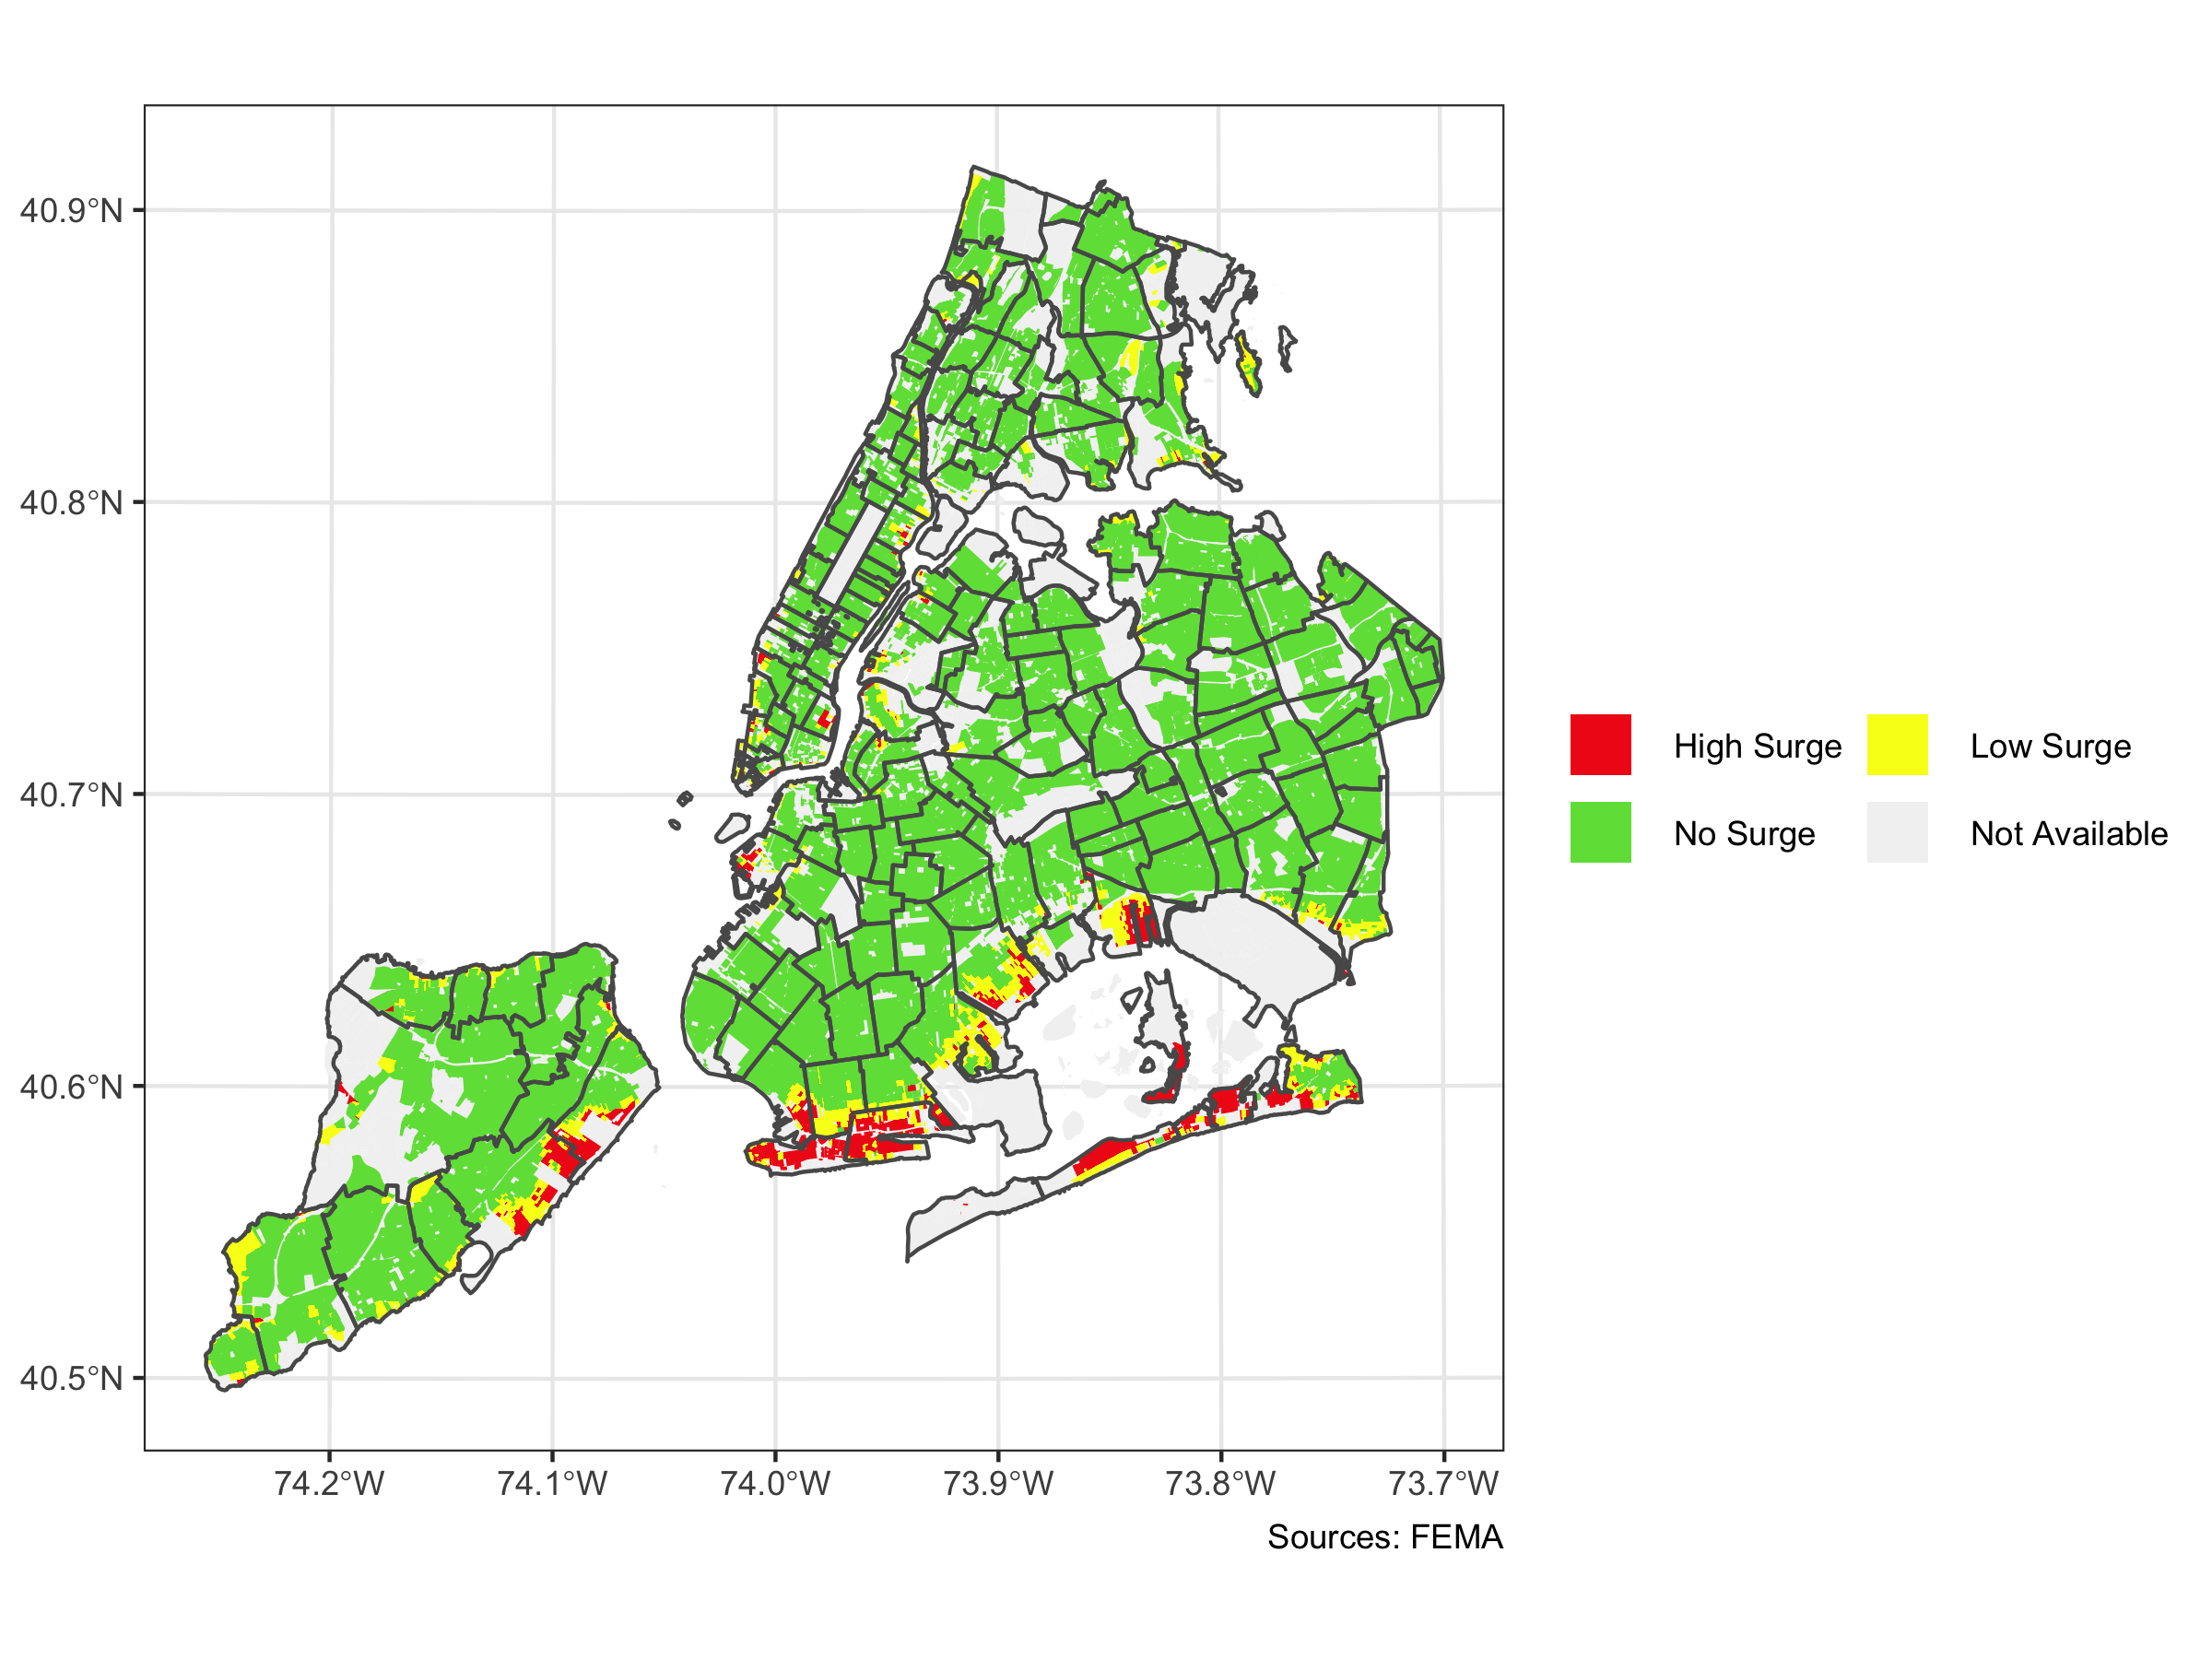
\includegraphics[scale = 0.22]{Samples/maps_zipcodeall.png}
\label{fig:zipmap}
\end{figure}

\clearpage
\begin{figure}[h!]
\begin{center}
\caption{High, Low and No Surge Blocks across the Flood Zone}
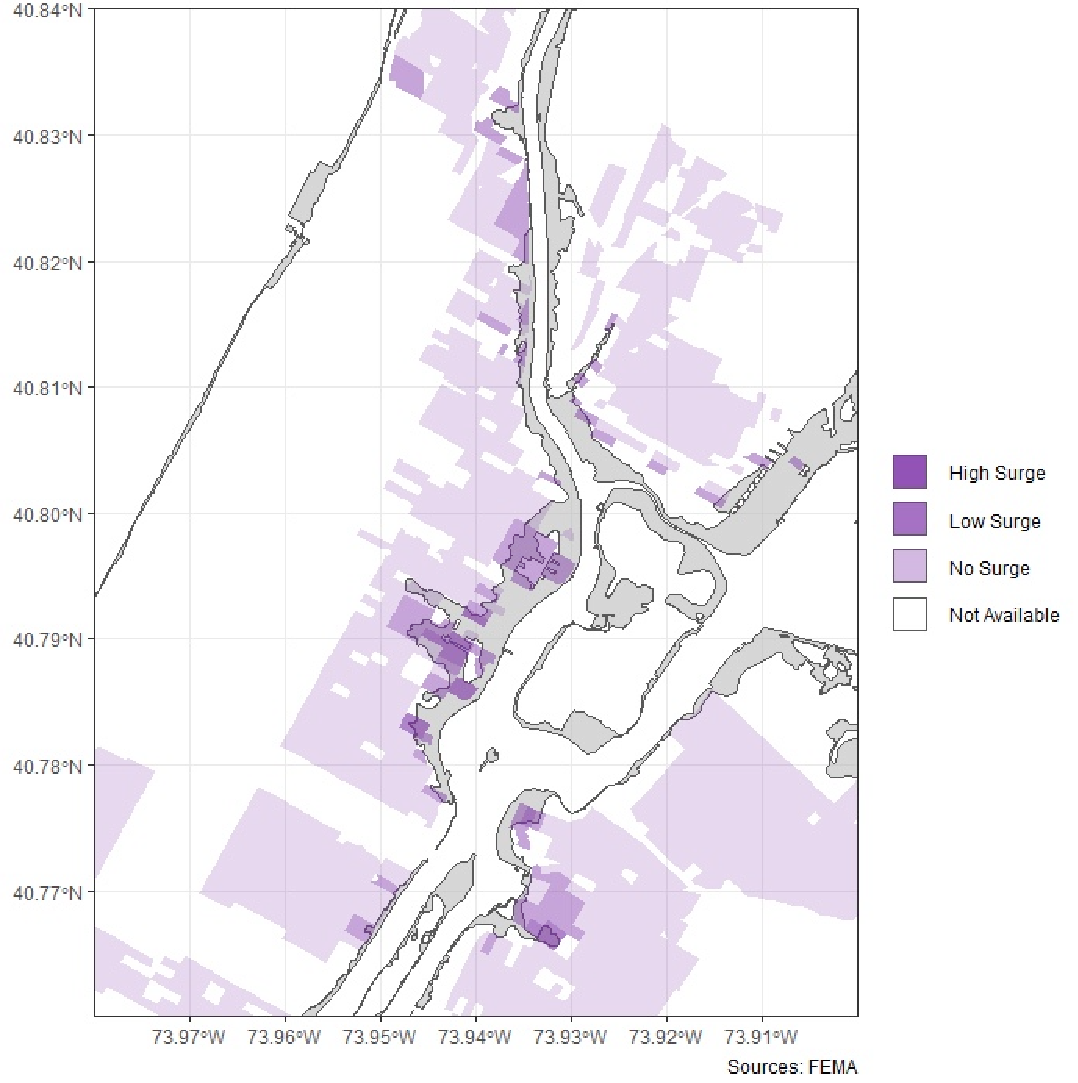
\includegraphics[scale = 0.55]{Samples/ues2.1.pdf}
\label{fig:ues}
\end{center}
\end{figure}

\begin{figure}[h!]
\caption{Percentage of Plot Incurred Major Damage by Surge Height}
\label{fig:damsurge}
\begin{center}
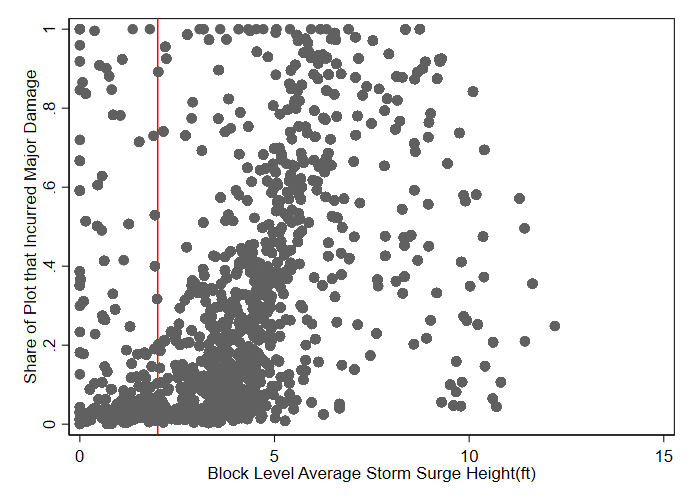
\includegraphics[scale = 0.41]{Damage/D1 scatter_damage.png}
\label{fig:scatdam}
\end{center}
\end{figure}

\begin{figure}[h!]
\caption{Composition of StreetEasy Sample over Time}
\begin{center}
\begin{subfigure}[b]{0.7\textwidth}
\caption{Number of Listings by Borough over Time}
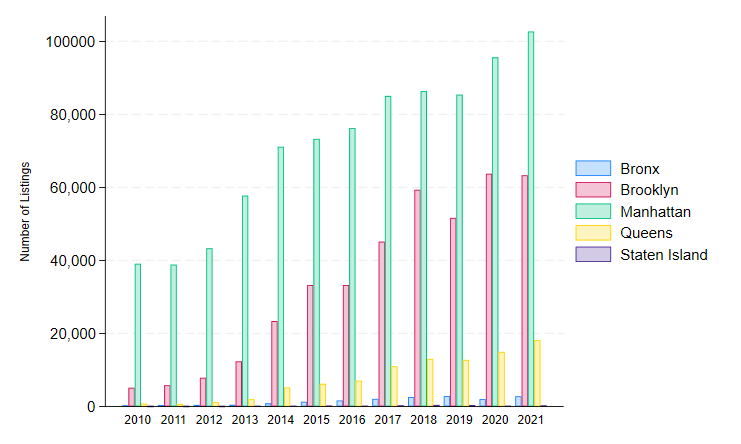
\includegraphics[scale = 0.6]{Samples/R7 SE Composition over Time.png}
\label{fig:seborough}
\end{subfigure}
\hfill
\begin{subfigure}[b]{0.7\textwidth}
\caption{Share of Listings by Building Type}
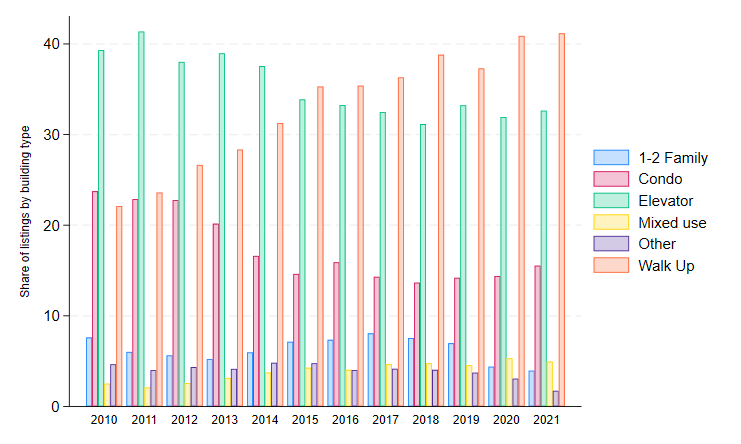
\includegraphics[scale = 0.6]{Samples/R7 SE Building Type over time.png}
\label{fig:sebuild}
\end{subfigure}
\end{center}
\end{figure}

\begin{figure}[h!]
\caption{Dispersion of StreetEasy Sample over Time}
\begin{center}
\begin{subfigure}[b]{0.78\textwidth}
\caption{StreetEasy Sample in 2011}
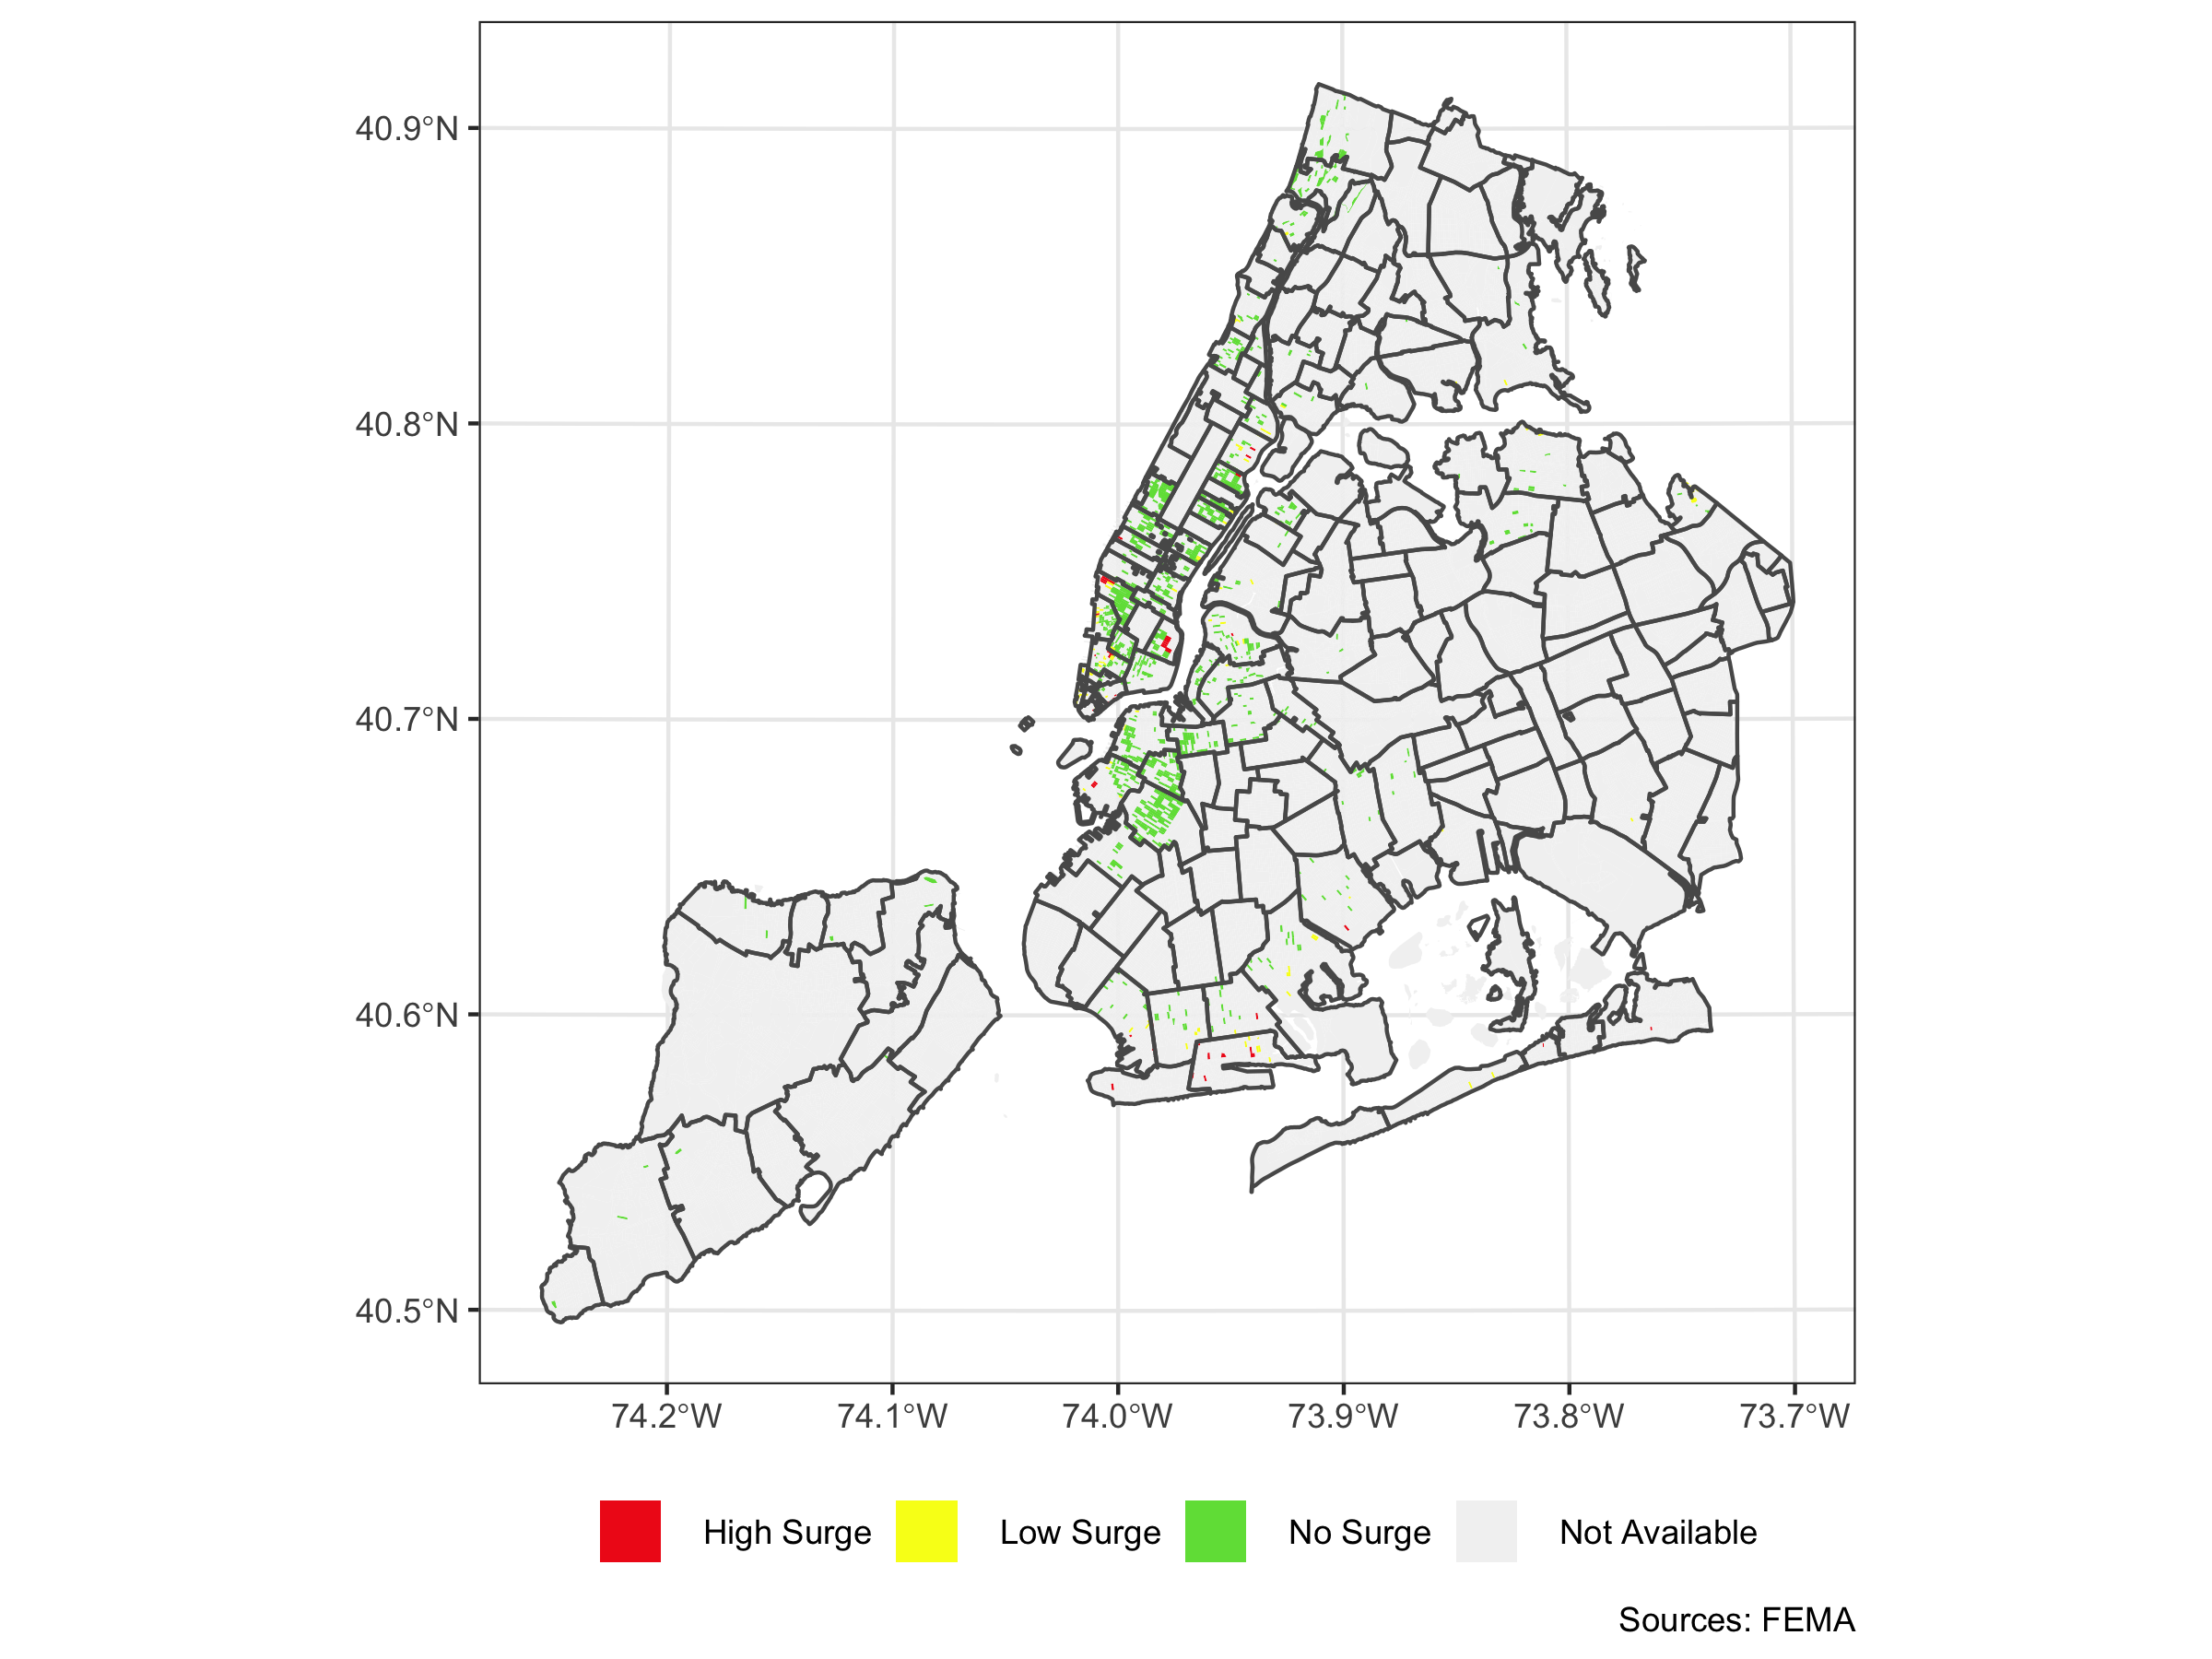
\includegraphics[scale = 0.17]{Samples/maps_zipcodestreet11.png}
\label{fig:2011sesample}
\end{subfigure}
\hfill
\begin{subfigure}[b]{0.5\textwidth}
\caption{StreetEasy Sample Across Full Time Period}
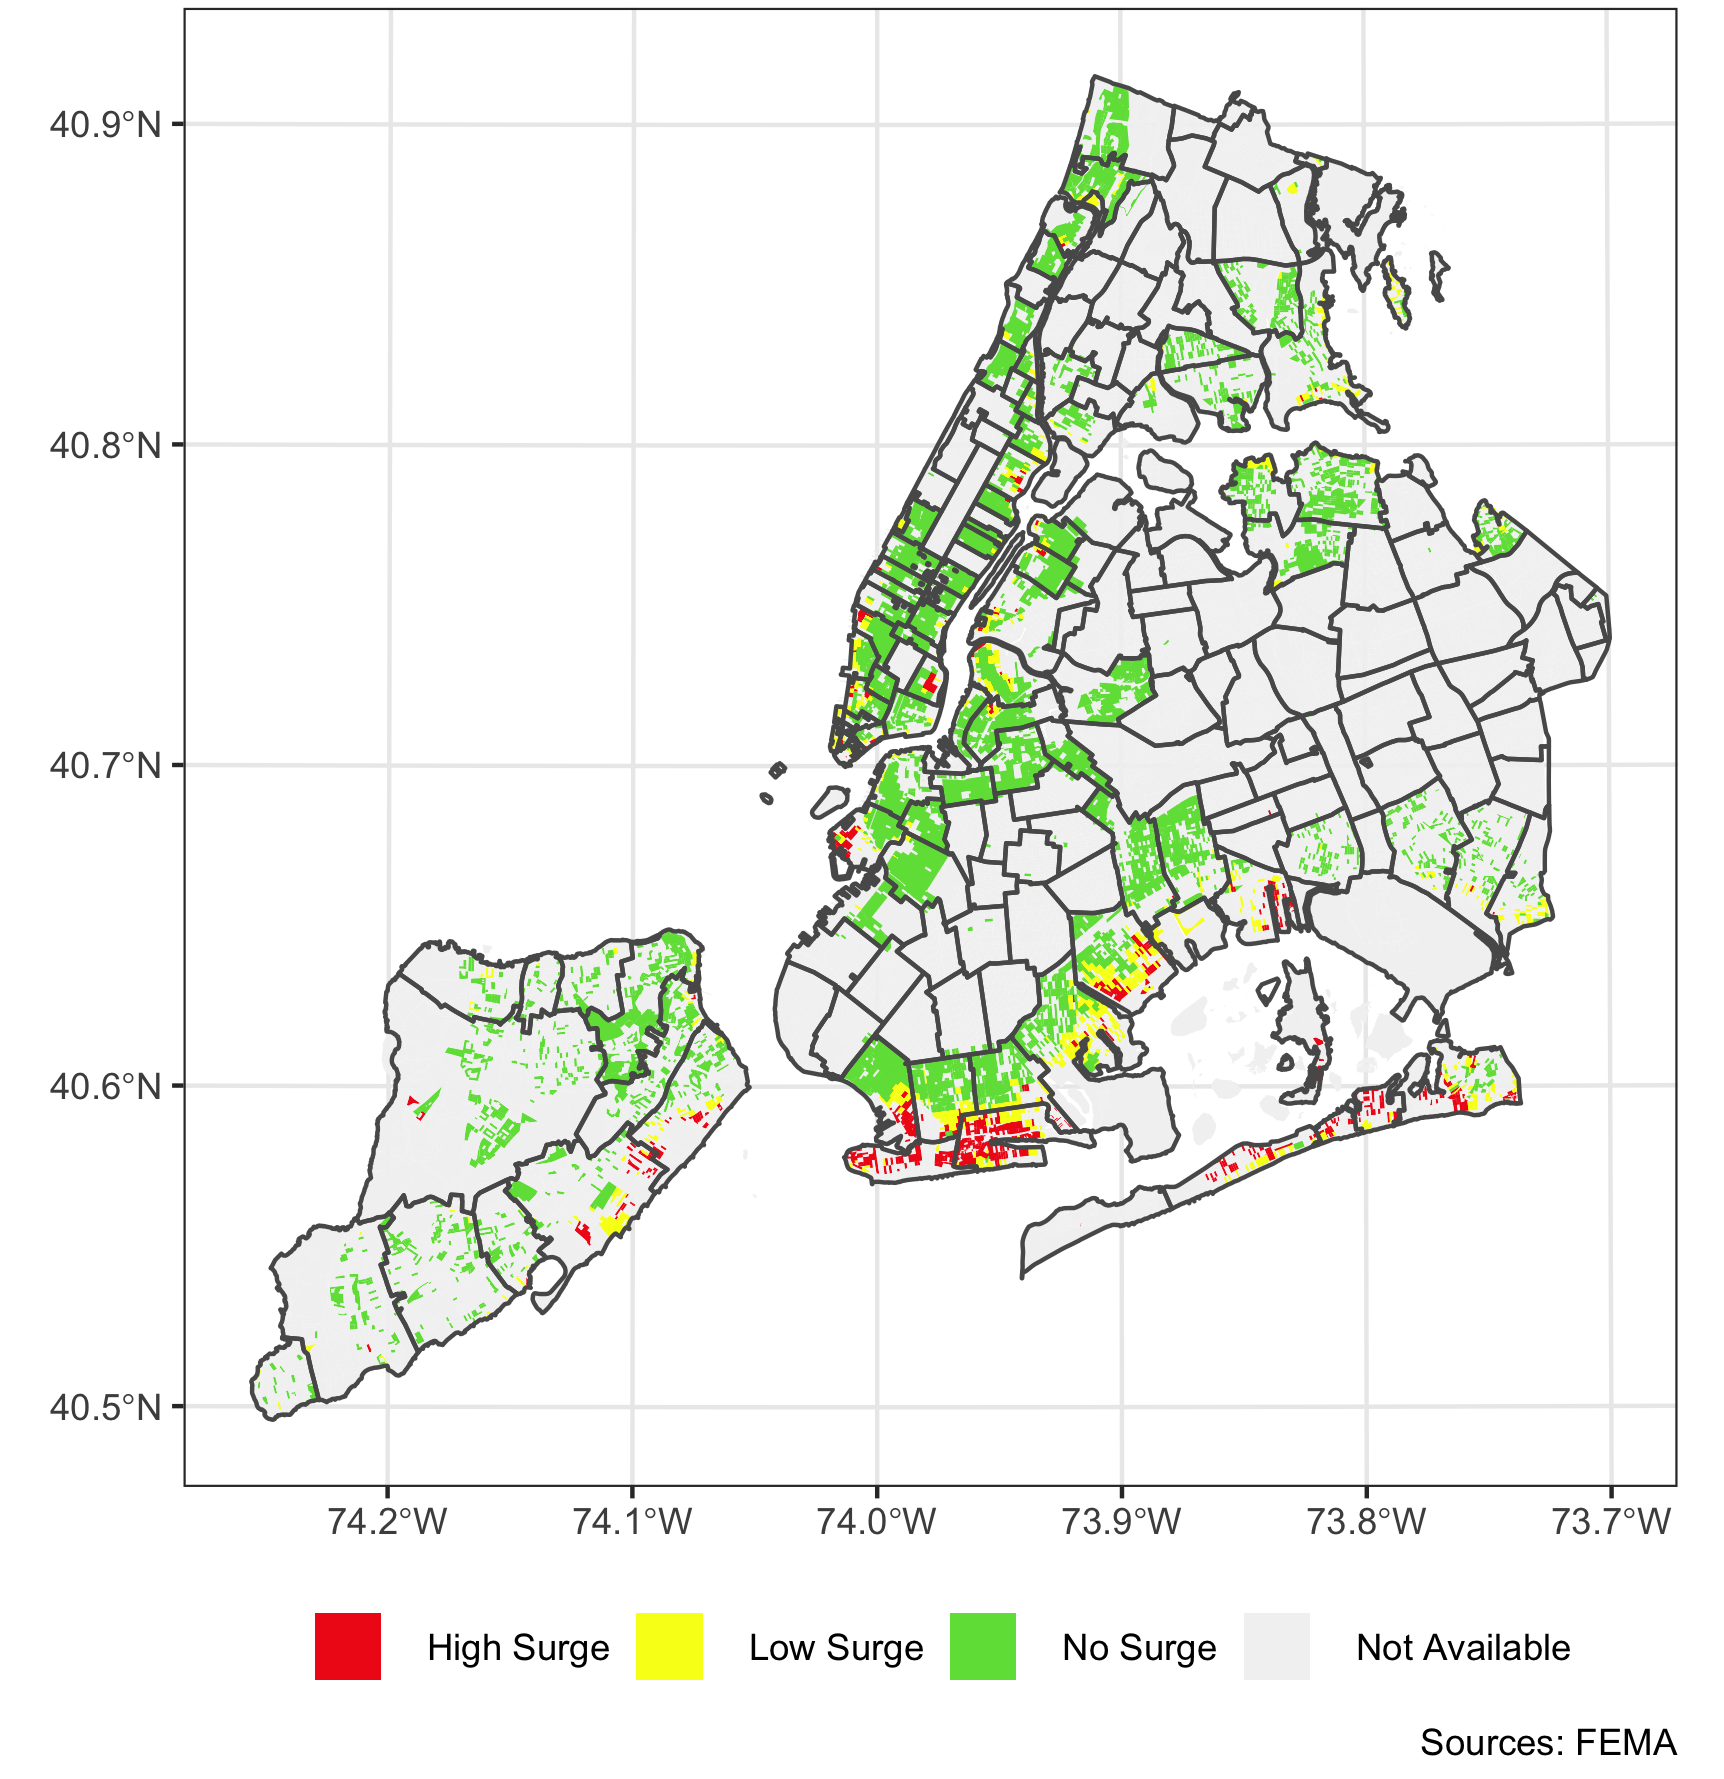
\includegraphics[scale = 0.17]{Samples/maps_zipcodestreet.png}
\label{fig:fullsesample}
\end{subfigure}
\end{center}
\end{figure}

\begin{figure}[h!]
\caption{Annual Change in Average Rents Over Time}
\label{fig:damsurge}
\begin{center}
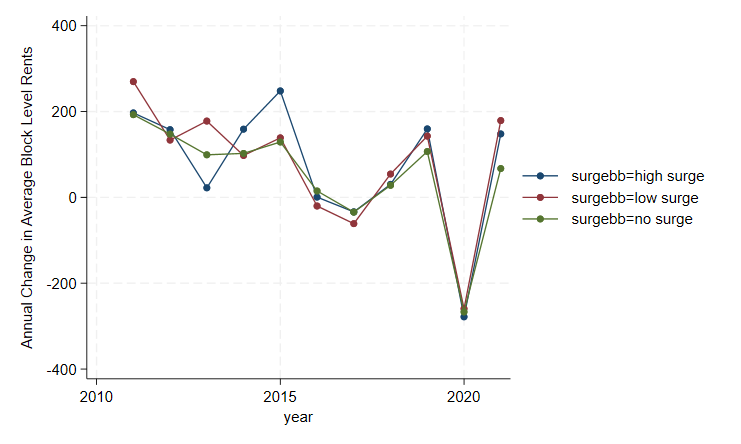
\includegraphics[scale = 0.5]{Samples/R7 SE Rent Change Over Time.png}
\label{fig:rentchange}
\end{center}
\end{figure}

\begin{figure}[h!]
\begin{center}
\caption{Impact of Hurricane Sandy on Asking Rents}
\begin{subfigure}[b]{0.6\textwidth}
\caption{Average Rents in High Surge Areas (Table \ref{tab:marketrents}, Column 1)}
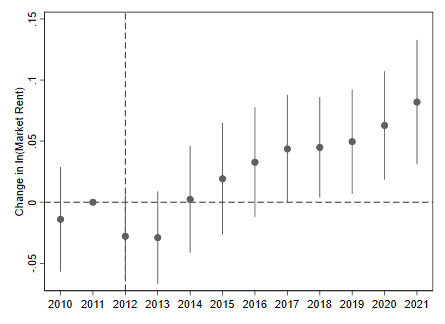
\includegraphics[scale = 0.6]{Street Easy Rents/R7 High Surge Rent Impacts_nohed.png}
\label{fig:highsurgemkt}
\end{subfigure}
\hfill
\begin{subfigure}[b]{0.6\textwidth}
\caption{Average Rents in High Surge Areas, controlling for age of building (Table \ref{tab:marketrents}, Column 2) }
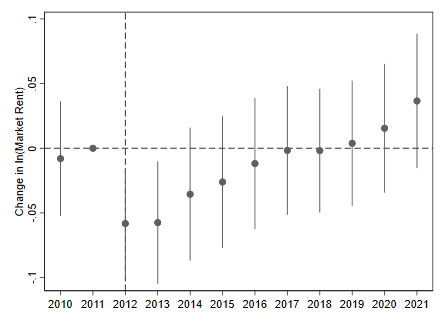
\includegraphics[scale = 0.6]{Street Easy Rents/R7 High Surge Rent Impacts_nohed_addage.png}
\label{fig:highsurgemktage}
\end{subfigure}
\hfill
\begin{subfigure}[b]{0.6\textwidth}
\caption{Average Rents in High Surge Areas, all controls (Table \ref{tab:marketrents}, Column 3)}
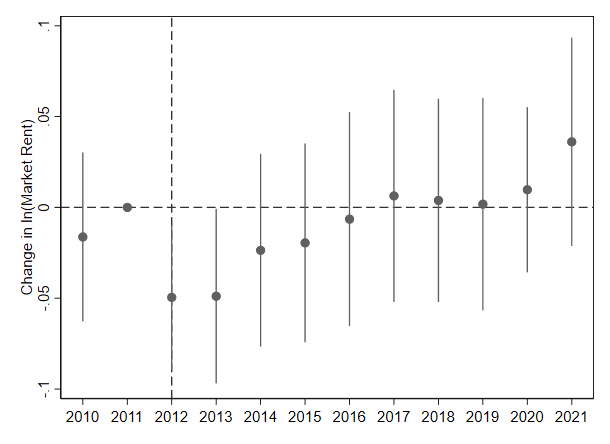
\includegraphics[scale = 0.45]{Street Easy Rents/R7 High Surge Rent Impacts_8_1.png}
\label{fig:highsurgemktcontrols}
\end{subfigure}
\end{center}
\end{figure}



% \begin{figure}[h!]
% \begin{center}
% \caption{Impacts on the Share of Buildings with Demolition, New Building and Renovation Permits}
% \label{fig:newbuilddemo}
% \begin{subfigure}[b]{0.4\textwidth}
% \caption{Demolition Permits}
% 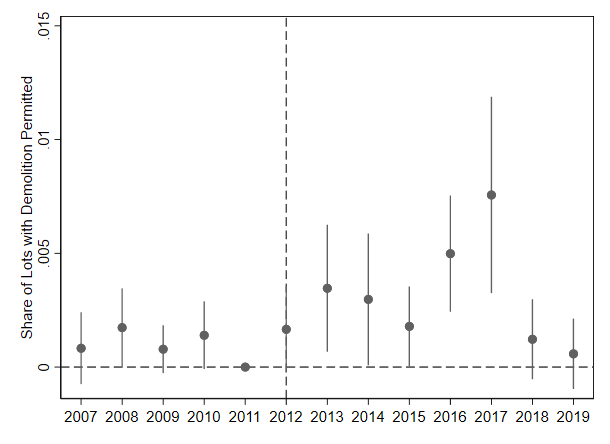
\includegraphics[scale = 0.4]{New Construction/R12 Demolitions Permitted.png}
% \label{fig:demo}
% \end{subfigure}
% \hfill
% \begin{subfigure}[b]{0.4\textwidth}
% \caption{New Building Permits}
% 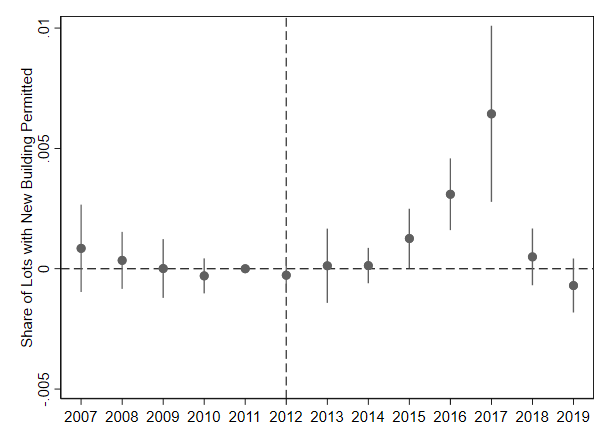
\includegraphics[scale = 0.4]{New Construction/R12 New Buildings Permitted.png}
% \label{fig:newbuild}
% \end{subfigure}
% \begin{subfigure}[b]{0.4\textwidth}
% \caption{Renovation Permits}
% 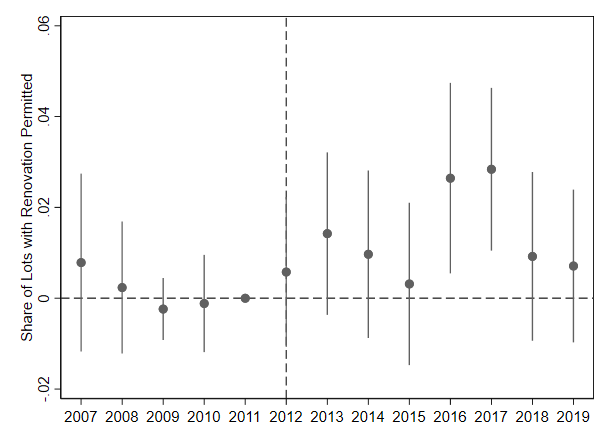
\includegraphics[scale = 0.4]{New Construction/R12 Renovations Permitted.png}
% \label{fig:renopermit}
% \end{subfigure}
% \hfill

% \end{center}
% \end{figure}

% \begin{figure}[h!]
% \begin{center}
% \caption{Asking Rents in High Surge Areas: all controls except age}
% \begin{subfigure}[b]{0.4\textwidth}
% \caption{Full Sample}
% 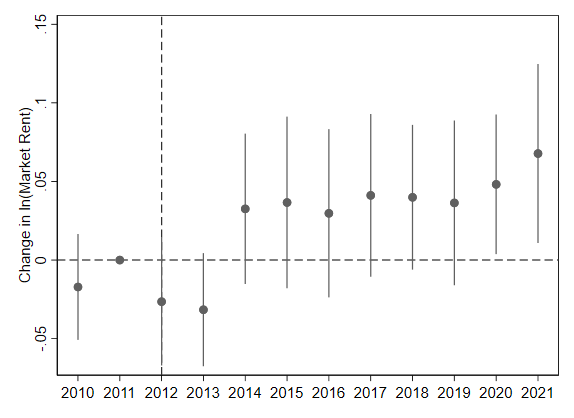
\includegraphics[scale = 0.4]{Street Easy Rents/R7 High Surge Rent Impacts.png}
% \label{fig:justnoage}
% \end{subfigure}
% \hfill
% \begin{subfigure}[b]{0.4\textwidth}
% \caption{Buildings built before 2012}
% 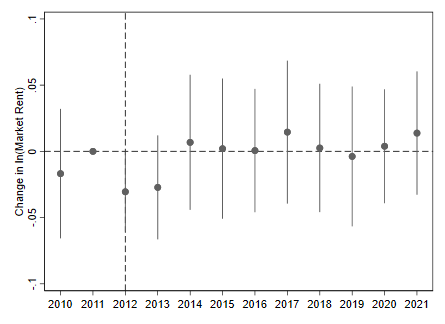
\includegraphics[scale = 0.5]{Street Easy Rents/R7 High Surge Rent Impacts_pre2013noage.png}
% \label{fig:nopost2012}
% \end{subfigure}
% \hfill
% \end{center}
% \end{figure}

% \begin{figure}[h!]
% \caption{Differential High Surge Rental Impacts for "Newer" Buildings: built since 2001}
% \begin{center}
% 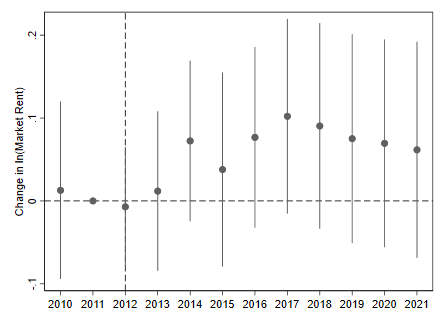
\includegraphics[scale = 0.6]{Street Easy Rents/R18 High Surge Newer_rentlevel.png}
% \label{fig:triplepost2001}
% \end{center}
% \end{figure}

\begin{figure}[h!]
\begin{center}
\caption{Quality-adjusted Rent Impacts by Neighborhood Income}
\begin{subfigure}[b]{0.4\textwidth}
\caption{At or Below Median Income}
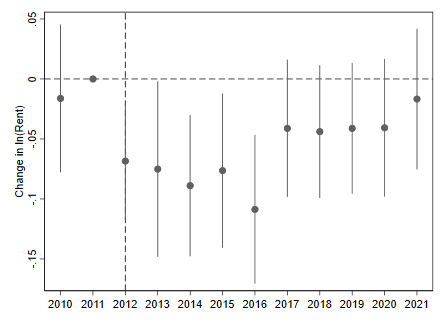
\includegraphics[scale = 0.5]{Street Easy Rents/Income Heterogeneity/R18 High Surge LowIncome_tract.png}
\label{fig:highinc}
\end{subfigure}
\hfill
\begin{subfigure}[b]{0.4\textwidth}
\caption{Above Median Income}
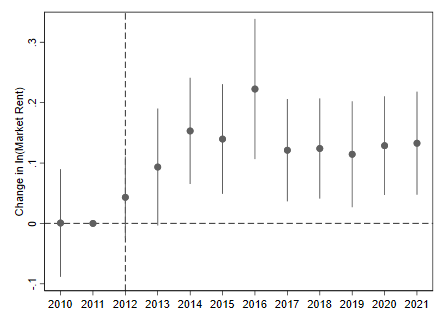
\includegraphics[scale = 0.5]{Street Easy Rents/Income Heterogeneity/R18 High Surge HighIncome_tract.png}
\label{fig:lowinc}
\end{subfigure}
\hfill
\end{center}
\end{figure}

\begin{figure}[h!]
\begin{center}
\caption{Impacts on the Share of Lots with Renovation Permits by Neighborhood Income}
\begin{subfigure}[b]{0.4\textwidth}
\caption{At or Below Median Income}
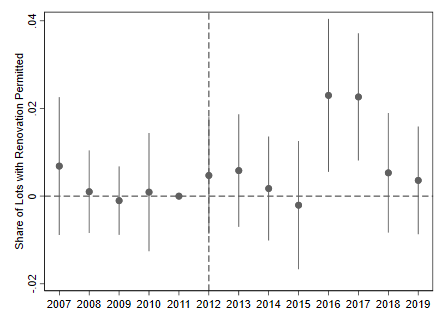
\includegraphics[scale = 0.5]{New Construction/R12 Renovations Permitted_lowincome.png}
\label{fig:highincren}
\end{subfigure}
\hfill
\begin{subfigure}[b]{0.4\textwidth}
\caption{Above Median Income}
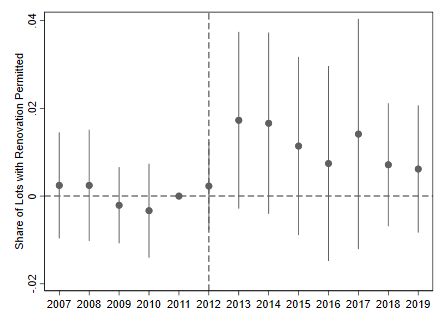
\includegraphics[scale = 0.5]{New Construction/R12 Renovations Permitted_highincome.png}
\label{fig:lowincren}
\end{subfigure}
\hfill
\end{center}
\end{figure}

\begin{figure}[h!]
\caption{Quality-adjusted Rental Impacts for Voucher Buildings}
\begin{center}
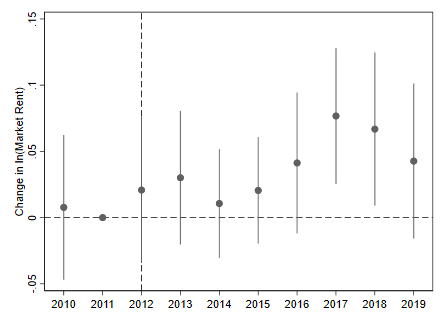
\includegraphics[scale = 0.6]{Street Easy Rents/R21 Voucher Build SE High Surge Rent Impacts.png}
\label{fig:sevouch}
\end{center}
\end{figure}



%%%% Voucher Rents

\begin{figure}
\begin{center}
\caption{Impact of Hurricane Sandy on Voucher Rents}
\begin{subfigure}[b]{0.4\textwidth}
\subcaption{High Surge Areas}
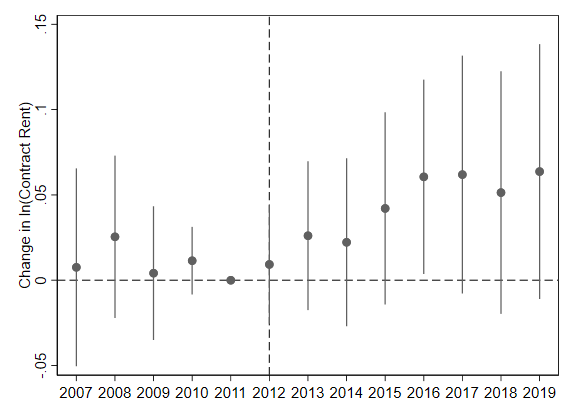
\includegraphics[scale=0.41]{Voucher Rents/R3 High Surge Voucher Rents_all vouchers.png}
\label{fig:highsurgevch}
\end{subfigure}
\hfill
\begin{subfigure}[b]{0.4\textwidth}
\subcaption{Low Surge Areas}
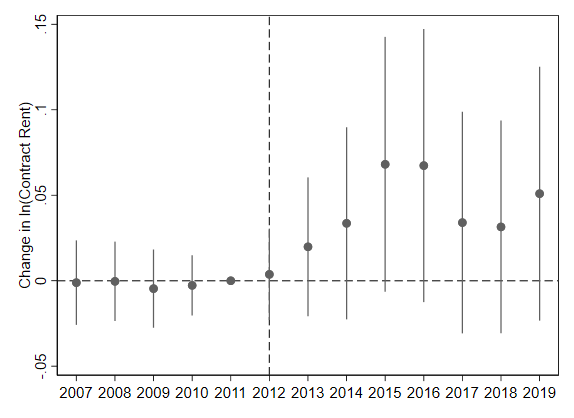
\includegraphics[scale=0.41]{Voucher Rents/R3 Low Surge Voucher Rent_all vouchers.png}
\label{fig:lowsurgevch}
\end{subfigure}
\begin{subfigure}[b]{0.4\textwidth}
\centering
\subcaption{High Surge, At/Below Median Income Neighborhoods}
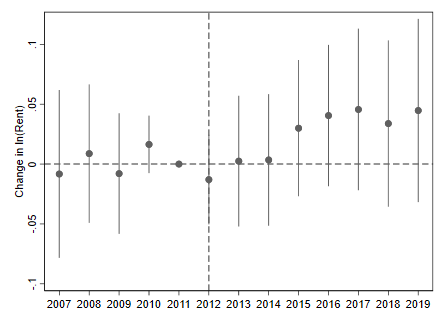
\includegraphics[scale=0.51]{Voucher Rents/R24 High Surge LowIncome_tract.png}
\label{fig:vouchlowinc}
\end{subfigure}
\hfill
\begin{subfigure}[b]{0.4\textwidth}
\subcaption{High Surge, Above Median Income Neighborhoods}
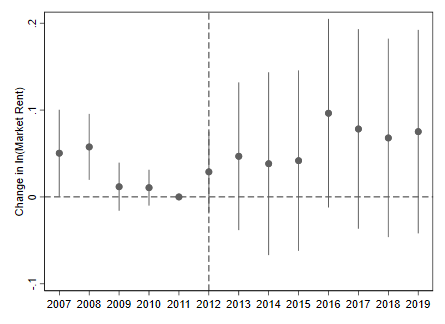
\includegraphics[scale=0.51]{Voucher Rents/R24 High Surge HighIncome_tract.png}
\label{fig:vouchhighinc}
\end{subfigure}
\end{center}
\end{figure}

\begin{figure}[h!]
\begin{center}
\caption{High Surge Voucher Rental Impacts by Tenure}
\begin{subfigure}[b]{0.4\textwidth}
\caption{Sitting Voucher Units}
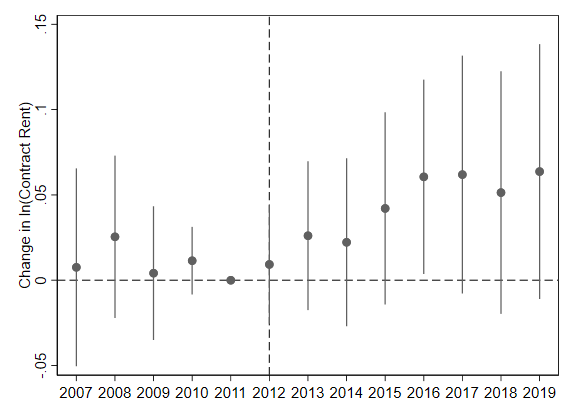
\includegraphics[scale = 0.41]{Voucher Rents/R3 High Surge Voucher Rents_all vouchers.png}
\label{fig:vouchsit}
\end{subfigure}
\hfill
\begin{subfigure}[b]{0.4\textwidth}
\caption{"New" Voucher Units}
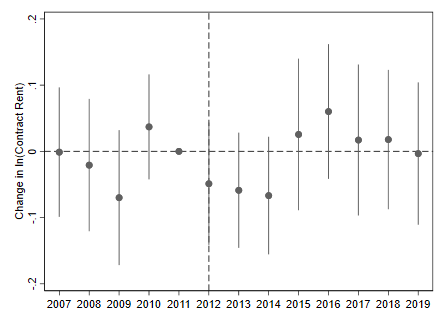
\includegraphics[scale = 0.55]{Voucher Rents/R3 High Surge Voucher Rents_newtobuild.png}
\label{fig:vouchnew}
\end{subfigure}
\end{center}
\end{figure}

\begin{figure}[h!]
\begin{center}
\caption{Share of Lots that Filed for Renovation Permits in Below Median Income Neighborhoods}
\begin{subfigure}[b]{0.4\textwidth}
\caption{Non Voucher Buildings}
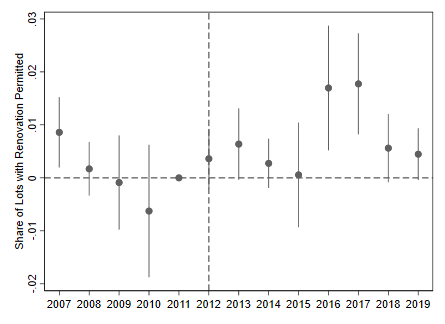
\includegraphics[scale = 0.55]{Renovations/R12 Renovations Permitted_nonvouchers_lowinc.png}
\label{fig:novouchreno}
\end{subfigure}
\hfill
\begin{subfigure}[b]{0.4\textwidth}
\caption{Voucher Buildings}
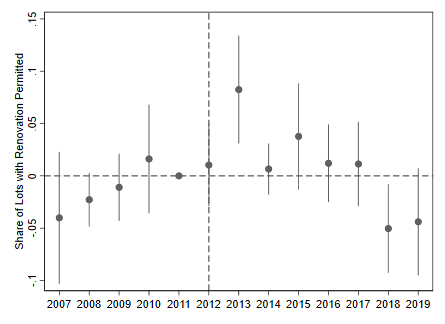
\includegraphics[scale = 0.55]{Renovations/R12 Renovations Permitted_vouchers_lowinc.png}
\label{fig:vouchreno}
\end{subfigure}
\end{center}
\end{figure}


\begin{figure}[h!]
\begin{center}
\caption{Differential Voucher Rental Impacts for 2013 Job Filings}
\begin{subfigure}[b]{0.4\textwidth}
\caption{Buildings that filed for 2013 renovation permit}
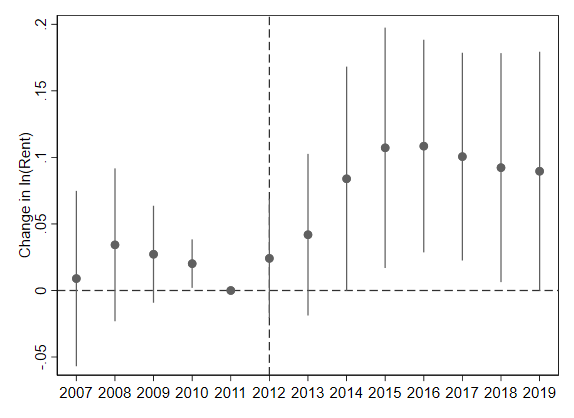
\includegraphics[scale = 0.41]{Renovations/R3.5 High Surge Jobs 2013_all vouchers.png}
\label{fig:highsurgevouchjob}
\end{subfigure}
\hfill
\begin{subfigure}[b]{0.4\textwidth}
\caption{Buildings that did not file for a 2013 permit}
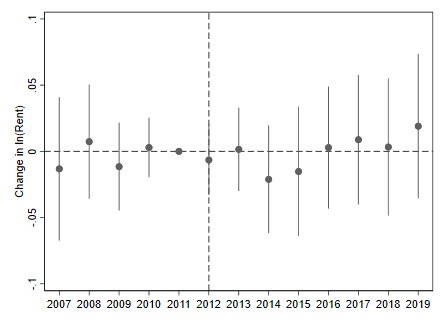
\includegraphics[scale = 0.55]{Renovations/R3.5 High Surge NO Jobs 2013_all vouchers.png}
\label{fig:vouchnojob}
\end{subfigure}
\end{center}
\end{figure}

%%% Voucher Incidence

\begin{figure}[h!]
\begin{center}
\caption{Impacts on Tenant and Housing Assistance Payments in High Surge Areas}
\begin{subfigure}[b]{0.4\textwidth}
\caption{Voucher Tenant Payments}
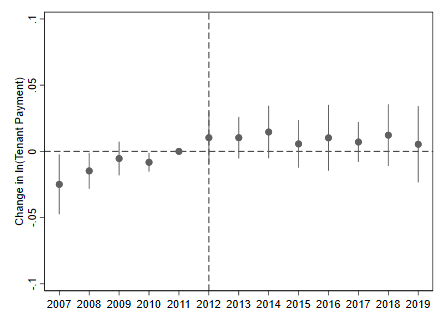
\includegraphics[scale = 0.48]{Voucher Incidence/R3 High Surge TTP_existing.png}
\label{fig:highsurgettp}
\end{subfigure}
\hfill
\begin{subfigure}[b]{0.4\textwidth}
\caption{Housing Assistance Payments}
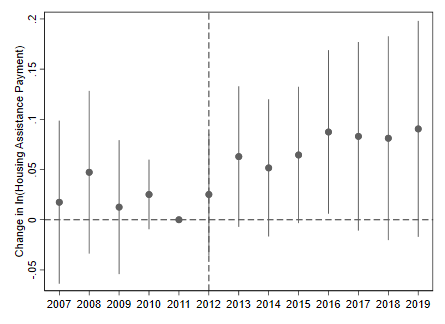
\includegraphics[scale = 0.48]{Voucher Incidence/R3 High Surge HAPs_existing.png}
\label{fig:highsurgehap}
\end{subfigure}
\end{center}
\end{figure}


% \begin{figure}[h!]
% \begin{center}
% \caption{Impacts on Existing Voucher Rents by Relation to Payment Standard in 2011, Job filings in 2013}
% \begin{subfigure}[b]{0.4\textwidth}
% \caption{At the Payment Standard}
% 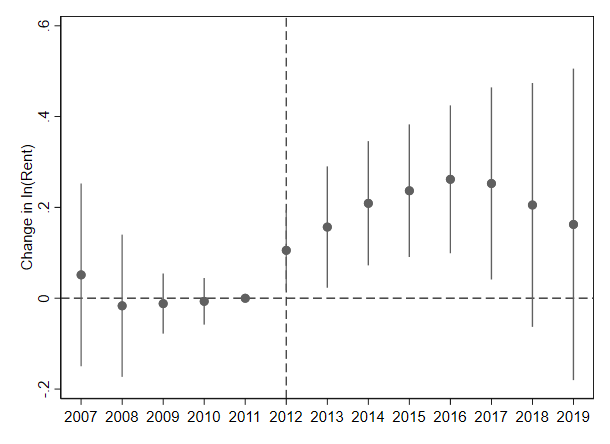
\includegraphics[scale = 0.4]{Voucher Incidence/R3 High Surge Jobs 2013_atps.png}
% \label{fig:highsurgeatps}
% \end{subfigure}
% \hfill
% \begin{subfigure}[b]{0.4\textwidth}
% \caption{Below Payment Standard}
% 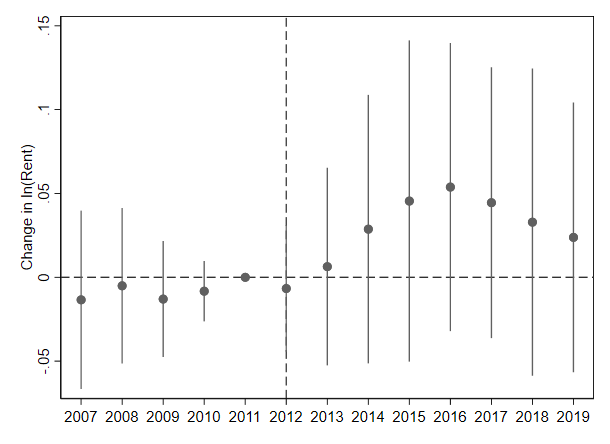
\includegraphics[scale = 0.4]{Voucher Incidence/R3 High Surge Jobs 2013_belowps.png}
% \label{fig:highsurgbeps}
% \end{subfigure}

% \begin{subfigure}[b]{0.4\textwidth}
% \caption{Above Payment Standard}
% 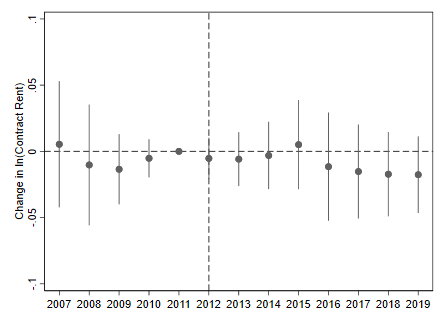
\includegraphics[scale = 0.6]{Voucher Incidence/R3 High Surge Voucher Rents_existingps.png}
% \label{fig:highsurgeps}
% \end{subfigure}
% \end{center}
% \end{figure}

% \begin{figure}[h!]
% \begin{center}
% \caption{Impacts on the Payment Standard (\$2021}
% \begin{subfigure}[b]{0.4\textwidth}
% \caption{Households Below the PS in 2011}
% 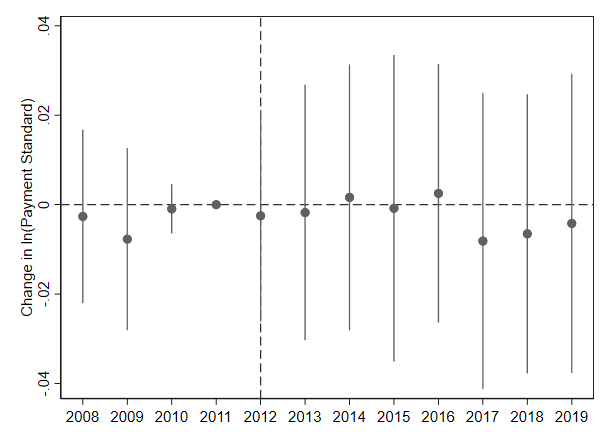
\includegraphics[scale = 0.41]{Voucher Incidence/R3 High Surge PS_below1.png}
% \label{fig:paystandb}
% \end{subfigure}
% \hfill
% \begin{subfigure}[b]{0.4\textwidth}
% \caption{Households at the PS in 2011}
% 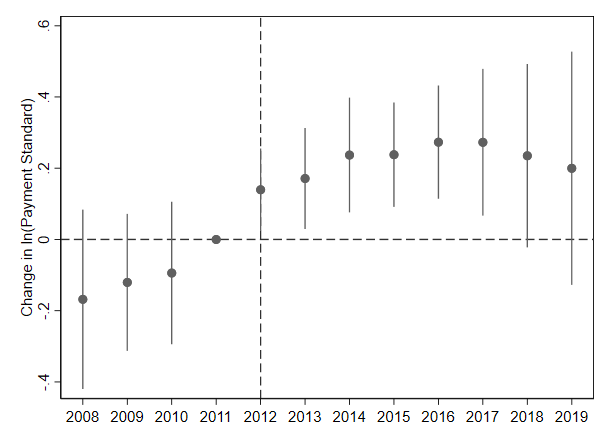
\includegraphics[scale = 0.41]{Voucher Incidence/R3 High Surge PS_at1.png}
% \label{fig:paystandat}
% \end{subfigure}
% \end{center}
% \end{figure}

%%% Robustness Figures


\begin{figure}[h!]
\begin{center}
\caption{Impacts on Sales Prices}
\begin{subfigure}[b]{0.4\textwidth}
\caption{High Surge Blocks}
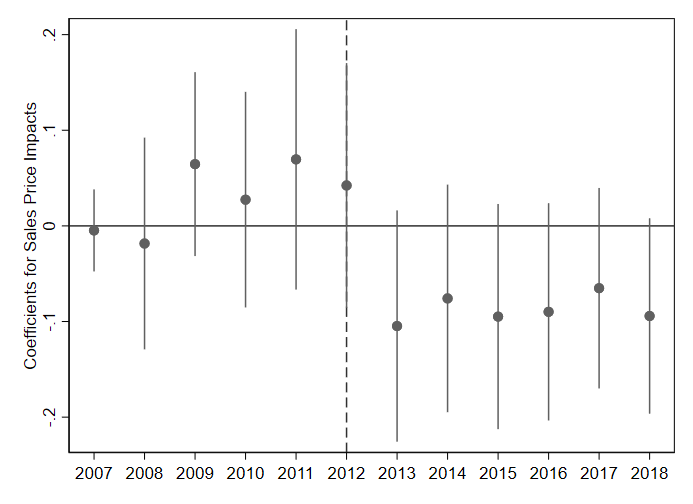
\includegraphics[scale = 0.35]{Robustness/Graph3c_high surge.png}
\label{fig:highsales}
\end{subfigure}f
\hfill
\begin{subfigure}[b]{0.4\textwidth}
\caption{Low Surge Blocks}
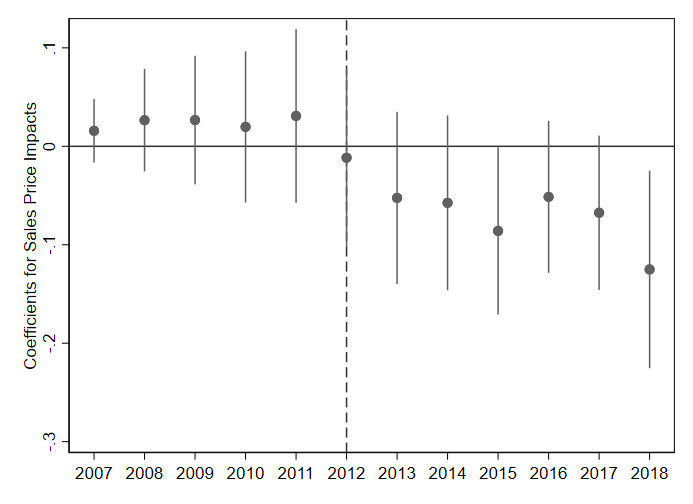
\includegraphics[scale = 0.35]{Robustness/Graph4c_low surge.png}
\label{fig:lowsales}
\end{subfigure}
\end{center}
\end{figure}

\begin{figure}[h!]
\begin{center}
\caption{Rental Impacts of Randomly Split Comparison Group}
\begin{subfigure}[b]{0.4\textwidth}
\caption{Market Rents}
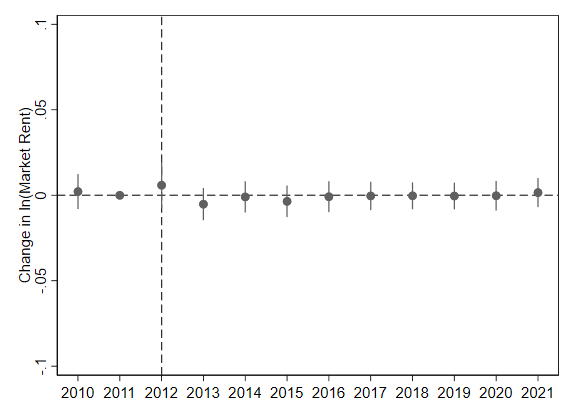
\includegraphics[scale = 0.41]{Robustness/R10 Street Easy Control Robust.png}
\label{fig:mktrobust}
\end{subfigure}
\hfill
\begin{subfigure}[b]{0.4\textwidth}
\caption{Voucher Rents}
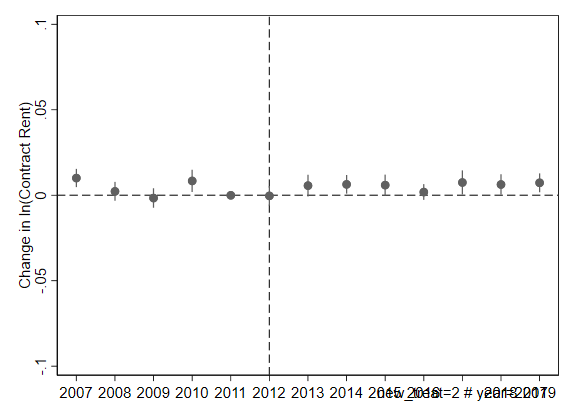
\includegraphics[scale = 0.41]{Robustness/R9 High Surge Voucher Rents_all vouchers_control robustness.png}
\label{fig:vouchrobust}
\end{subfigure}
\end{center}
\end{figure}


\clearpage
\section{Tables} 

\begin{table}[!htbp]
\begin{center}
\caption{\label{tab:marketsamp}Sample of Asking-Rent Listings by Surge Area}
\begin{tabular}{||c c c c c||} 
 \toprule
 %    \multicolumn{5}{1}{\textbf{Market Sample}}
 % \midrule
   2011 & High Surge & Low Surge & No Surge & Total \\ [0.5ex] 
\midrule
Listings & 2,070 & 6,078 & 37,647 & 45,795 \\
\hline
 Blocks & 110 & 222 & 2,043 & 2,375 \\  
 \hline
 Zip codes & 30  & 60 & 81 & 93 \\
 \midrule 
    2017 & High Surge & Low Surge & No Surge & Total \\ [0.5ex] 
\midrule
Listings & 6,042 & 16,265 & 123,306 & 145,613 \\
\hline
 Blocks & 330 & 501 & 3,900 & 4,731 \\  
 \hline
 Zip codes & 45  & 79 & 88 & 98 \\
\bottomrule
\end{tabular}
\end{center}
\end{table}



\begin{table}[!htbp]
%\includegraphics[scale=0.24]{housing vouch.jpg}
\centering
\caption{\label{tab:marketstats}Summary Statistics for Market Units in 2011 by Surge Level}
\begin{tabular}{l*{3}{c}}
\toprule
                &High Surge&Low Surge& No Surge\\
\midrule
\emph{Unit Level}&         &         &         \\
\addlinespace
No. Bedrooms        &     1.36&     1.25&     1.25\\
                &   (0.97)&   (0.89)&   (1.02)\\
\addlinespace
No. Bathrooms       &     1.25&     1.33&     1.22\\
                &   (0.53)&   (0.64)&   (0.59)\\
\addlinespace
No fee          &     0.44&     0.60&     0.31\\
                &   (0.50)&   (0.49)&   (0.46)\\
\addlinespace
Rent (in $2021)    &  4377.28&  5364.10&  4390.90\\
                &(3313.40)&(9058.12)&(4460.26)\\
\addlinespace
\emph{Building Level}&         &         &         \\
\addlinespace
No. Res. Units    &    47.83&    80.44&    41.39\\
                & (109.32)& (197.59)& (132.69)\\
\addlinespace
Building Age    &    74.86&    68.72&    84.66\\
                &  (40.78)&  (41.28)&  (32.44)\\
\addlinespace
\emph{Tract Level}&         &         &         \\
\addlinespace
Tract Pov Rate  &     0.17&     0.14&     0.18\\
                &   (0.08)&   (0.12)&   (0.13)\\
\addlinespace
Tract Share White&     0.53&     0.49&     0.46\\
                &   (0.26)&   (0.29)&   (0.30)\\
\addlinespace
Tract Share Black  &     0.11&     0.16&     0.15\\
                &   (0.19)&   (0.24)&   (0.23)\\
\addlinespace
Tract Share Hispanic &     0.16&     0.22&     0.25\\
                &   (0.14)&   (0.20)&   (0.23)\\
\addlinespace
Tract Share Asian  &     0.17&     0.10&     0.12\\
                &   (0.13)&   (0.12)&   (0.15)\\
\addlinespace
Tract Share College Degree  &     0.26&     0.24&     0.25\\
                &   (0.11)&   (0.12)&   (0.13)\\
\addlinespace
Tract Share Foreign Born &     0.44&     0.34&     0.32\\
                &   (0.18)&   (0.15)&   (0.15)\\
\addlinespace
Tract Med Rent (in $2021)&  1371.39&  1518.26&  1517.39\\
                & (467.23)& (479.22)& (499.75)\\
\bottomrule
\end{tabular}

\end{table}



\begin{table}[!htbp]
%\includegraphics[scale=0.24]{housing vouch.jpg}
\centering
\caption{\label{tab:marketrents}Impact of Hurricane Sandy on Market Rents}
{
\def\sym#1{\ifmmode^{#1}\else\(^{#1}\)\fi}
\begin{tabular}{l*{3}{c}}
\toprule
                    &\multicolumn{1}{c}{(1)}&\multicolumn{1}{c}{(2)}&\multicolumn{1}{c}{(3)}\\
                    &\multicolumn{1}{c}{Log Rent ($2021)}&\multicolumn{1}{c}{Log Rent ($2021)}&\multicolumn{1}{c}{Log Rent ($2021)}\\
\midrule
No. Bedrooms        &       0.165\sym{***}&       0.170\sym{***}&       0.168\sym{***}\\
                    &     (0.017)         &     (0.018)         &     (0.018)         \\
\addlinespace
high surge $\times$ post=1&       0.053\sym{***}&       0.018         &       0.021         \\
                    &     (0.018)         &     (0.021)         &     (0.020)         \\
\addlinespace
low surge $\times$ post=1&       0.010         &       0.010         &       0.016         \\
                    &     (0.022)         &     (0.019)         &     (0.020)         \\
\addlinespace
Building Age        &                     &      -0.005\sym{***}&      -0.004\sym{***}\\
                    &                     &     (0.000)         &     (0.000)         \\
\addlinespace
Building Age Sq     &                     &       0.000\sym{***}&       0.000\sym{***}\\
                    &                     &     (0.000)         &     (0.000)         \\
\addlinespace
No. Bathrooms       &                     &                     &       0.012         \\
                    &                     &                     &     (0.011)         \\
\addlinespace
No Broker Fee       &                     &                     &       0.006         \\
                    &                     &                     &     (0.005)         \\
\addlinespace
No. Res Units       &                     &                     &      -0.000         \\
                    &                     &                     &     (0.000)         \\
\addlinespace
Res Units Sq        &                     &                     &       0.000         \\
                    &                     &                     &     (0.000)         \\
\addlinespace
Subsidized housing  &                     &                     &      -0.016         \\
                    &                     &                     &     (0.014)         \\
\addlinespace
Number of Floors    &                     &                     &       0.008\sym{***}\\
                    &                     &                     &     (0.001)         \\
\addlinespace
Flood Zone          &                     &                     &       0.046\sym{**} \\
                    &                     &                     &     (0.019)         \\
\addlinespace
Constant            &       7.886\sym{***}&       8.122\sym{***}&       7.931\sym{***}\\
                    &     (0.025)         &     (0.025)         &     (0.028)         \\
\midrule
N                   &     1371538         &     1371538         &     1371536         \\
Age Controls        &                     &         X            &          X           \\
Zipcode * Year      &                     &           X         &           X         \\
Zipcode * Surge     &           X         &           X         &           X         \\

\tabnotes{4}{\textit{Notes:Regressions on log asking rents in \$2021. Column 1 includes on control for number of bedrooms, Column 2 adds age, Column 3 includes all controls. All models include zipcode by year and zipcode by surge level fixed effects.}. \textit{Clustered standard errors in parentheses.} * p $<$ 0.10 ** p $<$ 0.05 *** p $<$ 0.01 }

\end{table}

\newpage
\begin{table}[!htbp]
\begin{center}
\caption{\label{tab:vouchsamp}Sample of Voucher Holders by Surge Area, 2011}
\begin{tabular}{||c c c c c||} 
 \toprule
 %    \multicolumn{5}{1}{\textbf{Market Sample}}
 % \midrule
   2011 & High Surge & Low Surge & No Surge & Total \\ [0.5ex] 
\midrule
 Voucher Holders & 6,136 & 4,749 & 40,829 & 51,174 \\
  \hline
 Blocks & 394 & 499 & 4,093 & 4,986 \\ 
 \hline
 Zip codes & 37 & 79 & 92 & 96 \\
 \hline
\end{tabular}
\end{center}
\end{table}

\begin{table}[!htbp]
%\includegraphics[scale=0.24]{housing vouch.jpg}
\centering
\caption{\label{tab:vouchstats}Summary Statistics for Voucher Units in 2011 by Surge Level}
\begin{tabular}{l*{3}{c}}
\toprule
                &High Surge&Low Surge& No Surge\\
\midrule
\emph{Unit Level}&         &         &         \\
\addlinespace
HH Head Black      &     0.03&     0.05&     0.04\\
                &   (0.16)&   (0.22)&   (0.20)\\
\addlinespace
HH Head Hispanic    &     0.18&     0.22&     0.25\\
                &   (0.38)&   (0.41)&   (0.44)\\
\addlinespace
HH Head White      &     0.48&     0.35&     0.38\\
                &   (0.50)&   (0.48)&   (0.49)\\
\addlinespace
HH Head Over 65     &     0.46&     0.33&     0.28\\
                &   (0.50)&   (0.47)&   (0.45)\\
\addlinespace
Has Children  &     0.28&     0.36&     0.39\\
                &   (0.45)&   (0.48)&   (0.49)\\
\addlinespace
Contract Rent (in \$2021) &  1483.59&  1605.83&  1449.96\\
                & (546.51)& (844.68)& (488.48)\\
\addlinespace
HH Income/10000 (in \$2021)        &     1.97&     2.16&     1.85\\
                &   (1.39)&   (1.51)&   (1.18)\\
\addlinespace
Housing Assistance Payments (in \$2021)        &  1026.11&  1126.68&  1065.66\\
                & (506.63)& (808.20)& (475.51)\\
\addlinespace
Tenant Rent Portion (in \$2021)        &   490.37&   532.59&   445.97\\
                & (352.43)& (383.85)& (289.28)\\
\addlinespace
Share Above Payment Standard          &     0.04&     0.05&     0.07\\
                &   (0.20)&   (0.22)&   (0.25)\\
\addlinespace
Share At Payment Standard          &     0.38&     0.23&     0.13\\
                &   (0.48)&   (0.42)&   (0.33)\\
\addlinespace
Share 0-5\% Below PS       &     0.06&     0.09&     0.12\\
                &   (0.25)&   (0.29)&   (0.32)\\
\addlinespace
Share 5-10\% Below PS    &     0.08&     0.11&     0.13\\
                &   (0.27)&   (0.31)&   (0.34)\\
\addlinespace
Share 10-50\% Below PS     &     0.37&     0.48&     0.51\\
                &   (0.48)&   (0.50)&   (0.50)\\
\addlinespace
Share \>50% Below PS       &     0.06&     0.05&     0.04\\
                &   (0.24)&   (0.21)&   (0.20)\\
\addlinespace
\emph{Building Level}&         &         &         \\
\addlinespace
No. Res. Units        &   389.41&  1193.76&   142.83\\
                & (471.68)&(2413.30)& (342.67)\\
\addlinespace
Building Age    &    49.54&    55.75&    70.41\\
                &  (21.68)&  (29.30)&  (29.96)\\
\bottomrule
\end{tabular}

\end{table}



\begin{table}[!htbp]
%\includegraphics[scale=0.24]{housing vouch.jpg}
\centering
\caption{\label{tab:vouchstats2}Summary Statistics for Voucher Units in 2011 by Surge Level (Continued)}
\begin{tabular}{l*{3}{c}}
\toprule
                &High Surge&Low Surge& No Surge\\
\midrule
\emph{Tract Level}&         &         &         \\
\addlinespace
Tract Poverty Rate &     0.25&     0.23&     0.27\\
                &   (0.11)&   (0.15)&   (0.13)\\
\addlinespace
Tract Share White  &     0.42&     0.30&     0.27\\
                &   (0.34)&   (0.31)&   (0.31)\\
\addlinespace
Tract Share Black  &     0.30&     0.31&     0.24\\
                &   (0.25)&   (0.28)&   (0.23)\\
\addlinespace
Tract Share Hispanic&     0.20&     0.31&     0.40\\
                &   (0.15)&   (0.26)&   (0.27)\\
\addlinespace
Tract Share Asian  &     0.06&     0.06&     0.08\\
                &   (0.09)&   (0.10)&   (0.12)\\
\addlinespace
Tract Share College Degree&     0.17&     0.17&     0.15\\
                &   (0.09)&   (0.09)&   (0.09)\\
\addlinespace
Tract Share Foreign Born&     0.42&     0.34&     0.35\\
                &   (0.19)&   (0.14)&   (0.14)\\
\addlinespace
Tract Median Rent (in \$2021)&  1009.00&  1182.58&  1197.20\\
                & (349.23)& (312.86)& (334.01)\\
\bottomrule
\end{tabular}

\end{table}

\begin{table}[!htbp]
\begin{center}
\begin{threeparttable}
\caption{\label{tab:femadamage} FEMA Damage Assessment by Type of Alteration}
\begin{tabular}{||c c c c c||} 
 \toprule
 %    \multicolumn{5}{1}{\textbf{Market Sample}}
 % \midrule
    & A1 & A2 & A3 & Total \\ [0.5ex] 
\midrule
 Major Damage/Destroyed & 0.02  & 21.61 &  10.24 &   31.87 \\
 Minor Damage & 0.01 &  39.33 &  10.01 &   49.36 \\
 Affected   &0  &   3.17  &  8.78 &   11.95 \\
 No damage &0  &      0.20  &  6.61   &  6.82 \\
  Total    & 0.04  & 64.31 &  35.65  & 100.00 \\
 \hline
\end{tabular}
    \begin{tablenotes}
      \small
      \item This table shows the percentage of voucher holders in high surge areas by the FEMA Damage Assessment classification and the type of alteration permit the building filed for in 2013.
    \end{tablenotes}
  \end{threeparttable}
\end{center}
\end{table}



\begin{table}[!htbp]
%\includegraphics[scale=0.24]{housing vouch.jpg}
\centering
\caption{\label{tab:allvouchrents}All Voucher Rent Results}
{
\def\sym#1{\ifmmode^{#1}\else\(^{#1}\)\fi}
\begin{tabular}{l*{3}{c}}
\toprule
                    &\multicolumn{1}{c}{(1)}&\multicolumn{1}{c}{(2)}&\multicolumn{1}{c}{(3)}\\
                    &\multicolumn{1}{c}{Log Rent ($2021)}&\multicolumn{1}{c}{Log Rent ($2021)}&\multicolumn{1}{c}{Log Rent ($2021)}\\
\midrule
No. Bedrooms        &       0.160\sym{***}&       0.160\sym{***}&       0.156\sym{***}\\
                    &     (0.004)         &     (0.004)         &     (0.004)         \\
\addlinespace
high surge $\times$ post=1&       0.028         &       0.029         &       0.026         \\
                    &     (0.019)         &     (0.020)         &     (0.020)         \\
\addlinespace
low surge $\times$ post=1&       0.042\sym{**} &       0.039\sym{*}  &       0.042\sym{*}  \\
                    &     (0.021)         &     (0.022)         &     (0.023)         \\
\addlinespace
Building Age        &                     &      -0.002\sym{***}&      -0.002\sym{***}\\
                    &                     &     (0.001)         &     (0.001)         \\
\addlinespace
Building Age Sq     &                     &       0.000         &       0.000         \\
                    &                     &     (0.000)         &     (0.000)         \\
\addlinespace
No. Res Units       &                     &                     &      -0.000\sym{***}\\
                    &                     &                     &     (0.000)         \\
\addlinespace
Res Units Sq        &                     &                     &       0.000\sym{***}\\
                    &                     &                     &     (0.000)         \\
\addlinespace
No. of Floors       &                     &                     &       0.007\sym{**} \\
                    &                     &                     &     (0.003)         \\
\addlinespace
Subsidized housing  &                     &                     &      -0.096\sym{***}\\
                    &                     &                     &     (0.022)         \\
\addlinespace
Flood Zone          &                     &                     &      -0.088\sym{*}  \\
                    &                     &                     &     (0.048)         \\
\addlinespace
Constant            &       6.961\sym{***}&       7.060\sym{***}&       7.074\sym{***}\\
                    &     (0.009)         &     (0.016)         &     (0.022)         \\
\midrule
N                   &      681247         &      680663         &      680663         \\
Age Controls        &                     &           X         &           X         \\
All Other Controls  &                     &                     &           X          \\
Zipcode * Year      &           X         &           X         &           X         \\
Zipcode * Surge     &           X         &           X         &           X         \\
\tabnotes{4}{\textit{Notes:}Regressions estimated on repeated cross-section of all voucher units in the program during the time period. \textit{Standard errors in parentheses.} * p $<$ 0.10 ** p $<$ 0.05 *** p $<$ 0.01 }

\end{table}


\begin{table}[!htbp]
%\includegraphics[scale=0.24]{housing vouch.jpg}
\centering
\caption{\label{tab:NOPV stats}NOPV Summary Statistics (2005)}
\begin{tabular}{l*{3}{c}}
\toprule
                &High Surge&Low Surge& No Surge\\
\midrule
Building Age   &    74.53&    76.92&    80.49\\
                &  (26.81)&  (24.38)&  (19.73)\\
\addlinespace
Number of Res. Units        &    61.60&    54.94&    28.04\\
                & (142.31)& (325.42)&  (85.97)\\
\addlinespace
Number of Floors       &     6.03&     5.34&     4.89\\
                &   (4.50)&   (4.68)&   (3.28)\\
\addlinespace
Monthly Rental Income/Unit (\$2021) &  1768.16&  1658.86&  1618.50\\
                &(1232.35)&(1568.16)&(1396.65)\\
\midrule
  Number of buildings              &   687&  1639& 29,562\\
\bottomrule
\end{tabular}

\end{table}

\begin{table}[!htbp]
%\includegraphics[scale=0.24]{housing vouch.jpg}
\centering
\caption{\label{tab:NOPV res}Key Coefficients for NOPV DID High Surge Estimates}
{
\def\sym#1{\ifmmode^{#1}\else\(^{#1}\)\fi}
\begin{tabular}{l*{2}{c}}
\toprule
                    &\multicolumn{1}{c}{(1)}&\multicolumn{1}{c}{(2)}\\
                    &\multicolumn{1}{c}{\thead{Log Monthly Income/Unit \\(\$2021)}}&\multicolumn{1}{c}{\thead{Log Monthly Income/Unit \\ (\$2021)}}\\
\midrule
high surge $\times$ post=1&      -0.012         &              \\
                    &     (0.015)         &              \\
\addlinespace
high surge $\times$ post=1 $\times$ high\_rent=1&                     &       0.029         \\
                    &                     &     (0.041)         \\
                    \addlinespace
high surge $\times$ post=1 $\times$ low\_rent=1&                     &       -0.024         \\
                    &                     &     (0.032)         \\
\midrule
Zipcode * Year      &           X          &         X            \\
Zipcode * Surge     &       X              &        X             \\
N                   &      312567         &      312567         \\
\bottomrule
\multicolumn{3}{l}{\footnotesize Standard errors in parentheses}\\
\multicolumn{3}{l}{\footnotesize \sym{*} \(p<0.10\), \sym{**} \(p<0.05\), \sym{***} \(p<0.01\)}\\
\end{tabular}
}

\end{table}


% \begin{table}[!htbp]
% %\includegraphics[scale=0.24]{housing vouch.jpg}
% \centering
% \caption{\label{tab:vouchrents}Existing Voucher Rent Results}
% {
\def\sym#1{\ifmmode^{#1}\else\(^{#1}\)\fi}
\begin{tabular}{l*{3}{c}}
\toprule
                    &\multicolumn{1}{c}{(1)}&\multicolumn{1}{c}{(2)}&\multicolumn{1}{c}{(3)}\\
                    &\multicolumn{1}{c}{ln\_rent}&\multicolumn{1}{c}{ln\_rent}&\multicolumn{1}{c}{ln\_rent}\\
\midrule
presence\_child      &       0.006\sym{***}&       0.006\sym{***}&       0.006\sym{***}\\
                    &     (0.001)         &     (0.001)         &     (0.001)         \\
\addlinespace
head\_black          &      -0.004         &      -0.004         &      -0.004         \\
                    &     (0.004)         &     (0.004)         &     (0.004)         \\
\addlinespace
head\_white          &      -0.004\sym{*}  &      -0.004\sym{*}  &      -0.004\sym{*}  \\
                    &     (0.002)         &     (0.002)         &     (0.002)         \\
\addlinespace
NUM\_BEDRM\_CNT       &       0.122\sym{***}&       0.122\sym{***}&       0.122\sym{***}\\
                    &     (0.006)         &     (0.006)         &     (0.006)         \\
\addlinespace
head\_65\_over        &       0.000         &       0.000         &       0.000         \\
                    &     (0.002)         &     (0.002)         &     (0.002)         \\
\addlinespace
unitsres            &       0.000         &       0.000         &       0.000         \\
                    &     (0.000)         &     (0.000)         &     (0.000)         \\
\addlinespace
unitsressq          &      -0.000\sym{*}  &      -0.000         &      -0.000         \\
                    &     (0.000)         &     (0.000)         &     (0.000)         \\
\addlinespace
flood\_zone          &       0.002         &       0.000         &       0.001         \\
                    &     (0.017)         &     (0.017)         &     (0.016)         \\
\addlinespace
high surge $\times$ post=1&       0.023\sym{***}&       0.023\sym{***}&       0.023\sym{***}\\
                    &     (0.008)         &     (0.008)         &     (0.008)         \\
\addlinespace
low surge $\times$ post=1&       0.014         &       0.014         &       0.014         \\
                    &     (0.017)         &     (0.017)         &     (0.017)         \\
\addlinespace
building\_age        &                     &       0.000         &      -0.000         \\
                    &                     &     (0.000)         &     (0.000)         \\
\addlinespace
building\_age\_sq     &                     &      -0.000         &      -0.000         \\
                    &                     &     (0.000)         &     (0.000)         \\
\midrule
Zipcode * Year      &                     &                     &                     \\
Zipcode * Surge     &                     &                     &                     \\
N                   &      601459         &      601459         &      600884         \\
\bottomrule
\multicolumn{4}{l}{\footnotesize Standard errors in parentheses}\\
\multicolumn{4}{l}{\footnotesize \sym{*} \(p<0.10\), \sym{**} \(p<0.05\), \sym{***} \(p<0.01\)}\\
\end{tabular}
}

% \end{table}

\clearpage
\appendix

\section{Appendix}{\label{sec:AppA}
\setcounter{figure}{0}
\setcounter{table}{0}
\counterwithin{table}{section}
\counterwithin{figure}{section}

Below I discuss the results for further measures of heterogeneity associated with building age. 

\subsubsection{Building Height}
Since units on lower floors were more likely to be damaged by the storm surge than units on higher floors, it's possible that there was an increase in demand for taller buildings, specifically, if they were viewed as more storm resistant. Newer buildings do tend to be taller, however I find no evidence of an increase in rents for taller buildings independent of age. As Figure \ref{fig:tallage} shows, there is no increase in quality controlled rents for buildings above the median height built before the hurricane. 

\subsubsection{Renovations} {\label{sec:Renovations}
While new construction changed the composition of the rental stock in high surge areas, and therefore the average rents, there may also have been some heterogeneity in rental impacts among older buildings through renovations after the storm.  If landlords conducted renovations to repair damage and return their unit to its initial quality, we would not expect landlords to be able to pass on renovation costs into rents.  However, some research suggests that landlords enjoy monopoly pricing power power in New York City (\cite{watson_is_2021}), and, in the wake of a disaster, they may enjoy even more abnormal market power. In addition, if the landlord took the opportunity to improve the unit beyond its original condition, a well functioning market would allow those costs to be passed onto rents. 

Figure \ref{fig:mktnojob} plots the relative rental impacts for buildings in high surge areas that did not file for renovation permits in 2013 (r = 0) and \ref{fig:mktjob} plots the $\beta (s= high,r = 1)$ from equation \ref{eq:renov} which represent the differential impact for buildings that did file for permits in 2013-2015. Interestingly, while rents decreased initially for buildings that did not file for renovation permits in the 3 years after the hurricane, and slightly increased for those that did, neither impact is persistent throughout the period. 



% \subsubsection{Compositional Changes}
% It is possible that rents in newer, taller buildings that did not need renovations, were higher than in other buildings all along, and post storm, they comprised a greater share of the housing stock in high surge areas.  Specifically, landlords may have chosen not to invest in repairing damaged older buildings in high surge areas, and the units in these buildings, in turn, fell out of the rental stock. It's worth noting that at baseline, as Table \ref{tab:marketstats} shows, the buildings in high surge areas were younger than those in no surge area, and yet average rents were nearly the same.  Still, Figure \ref{fig:pre2000} shows an estimation of equation \ref{eq:rents} where the outcome is the share of buildings that were built before 2000. The coefficients depict the change in the share of older buildings in high surge areas relative to non-surge areas over time.  It is clear that the share of older buildings in high surge areas is decreasing over time relative to non-surge areas.  However, there does not appear to be a large impact from the hurricane itself, and magnitudes are relatively small and gradual, suggesting that this compositional change is most likely not the main driving factor behind the rather stark rent increases.


\subsubsection{Building Ownership}
If newer buildings are driving rental increases in high surge neighborhoods, potentially there is something different about the ownership of these buildings. Given the evidence that prices fell in affected areas (\cite{ellen_heterogeneity_2022}, \cite{ortega_rising_2018}), it is possible that certain buyers aimed to take advantage of the price discounts, bought rental properties and adjusted management practices to raise rents. Consistent with Ellen and Melterz (\citeyear{ellen_heterogeneity_2022}), I find no evidence of an increase in the share of lots or units sold in the years after the hurricane (Figure \ref{fig:sales}).  In addition, the main results are unaffected by dropping listings from properties that were sold in the last month of 2012, 2013 or 2014 (Figure \ref{fig:dropsale1214}).  

While I do not find evidence that landlord turnover is driving the rental increases, in future drafts of this paper, I will explore whether existing building ownership plays a role.  It's possible that the rental increases are a driven by a subset of landlord(s), or a certain type of landlord.  This effort is part of ongoing work on this paper.  

\subsubsection{Information}
While the flood zone is less likely to be a salient boundary for renters than homeowners, as discussed in Section \ref{sec:Theory}, it is still possible that households outside of the flood zone were less aware of the level of flood risk of their neighborhoods and that after the hurricane, renters in these neighborhoods updated their preferences accordingly: toward newer buildings they viewed as less prone to flood damage. The StreetEasy listings data prevents me from doing a full comparison of the impacts within and outside of the flood zone because in the pre-period I have less than 10 listings each year in the flood zone that did not experience surge\footnote{There are a substantial number of blocks that were in the flood zone that did not experience surge, but the buildings on these blocks do not appear to use StreetEasy.}.  However, roughly half of the listings in high surge areas are outside of the flood zone.  

When limiting the sample to those listings outside the flood zone, Figure \ref{fig:outsidefz} shows that the relative rental increases between high surge and no surge areas are even larger. Rents increased in high surge areas outside of the flood zone by 5\% relative to non surge areas outside the flood zone by 2014, and by 2021 they had increased by 10\%.  While these results clearly reflect the change in the composition of the rental stock in these neighborhoods, they may also present some initial evidence of renters updating their preferences.  Demand for units in newly constructed buildings, perhaps viewed as more flood-resistant, may have increased more in areas where residents were less aware of the riskiness of their neighborhoods at baseline.

However, updates to building requirements after the hurricane were limited to buildings that were located within either the flood zone boundaries that were in effect at the time of the hurricane (2007 FEMA FIRMS) or the boundaries that went into effect after the storm (2013 FEMA FIRMS). The most substantial restrictions required builders to move electrical equipment such as water heaters to floors above the basement, and to elevate their structures based on the base flood elevation designated by the FIRMS maps (\cite{nyc_building_code_new_2008}, \cite{nyc_department_of_buildings_rebuilding_2015}). I estimate the impacts separately for both flood zone boundaries and using a compiled measure of the flood zone boundary which uses the maximum riskiness designation across the two FIRMS maps, as builders were instructed to do by the city. In all 3 specifications, I find the stronger compositional effects outside the flood zone. 

\clearpage
\section{Appendix}{\label{sec:AppB}
\setcounter{figure}{0}
\setcounter{table}{0}
\counterwithin{table}{section}
\counterwithin{figure}{section}

\begin{table}[!htbp]
%\includegraphics[scale=0.24]{housing vouch.jpg}
\centering
\caption{\label{tab:surgelevs}Key Rental Impact Coefficients using Different Thresholds for High Surge}
{
\def\sym#1{\ifmmode^{#1}\else\(^{#1}\)\fi}
\begin{tabular}{l*{3}{c}}
\toprule
                    &\multicolumn{1}{c}{(1)}&\multicolumn{1}{c}{(2)}&\multicolumn{1}{c}{(3)}\\
                    &\multicolumn{1}{c}{Log Rent (2021\$)}&\multicolumn{1}{c}{Log Rent (2021\$)}&\multicolumn{1}{c}{Log Rent (2021\$)}\\
\midrule
high surge (\>1ft) $\times$ post=1&       0.030         &                     &                     \\
                    &     (0.025)         &                     &                     \\
\addlinespace
high surge (\>2ft) $\times$ post=1&                     &       0.051\sym{***}  &                     \\
                    &                     &     (0.018)         &                     \\
\addlinespace
high surge (\>3ft) $\times$ post=1&                     &                     &       0.049\sym{**}         \\
                    &                     &                     &     (0.023)         \\
\midrule
Zipcode * Year      &          X           &         X            &        X             \\
Zipcode * Surge     &           X          &          X           &         X            \\
N                   &     1371537         &     1371536         &     1371537         \\
\bottomrule
\multicolumn{4}{l}{\footnotesize Standard errors in parentheses}\\
\multicolumn{4}{l}{\footnotesize \sym{*} \(p<0.10\), \sym{**} \(p<0.05\), \sym{***} \(p<0.01\)}\\
\end{tabular}
}

\end{table}

\begin{table}[!htbp]
%\includegraphics[scale=0.24]{housing vouch.jpg}
\centering
\caption{\label{tab:surgelevs}Key Rental Impact Coefficients for High Surge Heterogeneity by Neighborhood Income}
{
\def\sym#1{\ifmmode^{#1}\else\(^{#1}\)\fi}
\begin{tabular}{l*{2}{c}}
\toprule
                    &\multicolumn{1}{c}{(1)}&\multicolumn{1}{c}{(2)}\\
                    &\multicolumn{1}{c}{Street Easy}&\multicolumn{1}{c}{Vouchers}\\
\midrule
high surge $\times$ post=1&      -0.055         &       0.030         \\
                    &     (0.034)         &     (0.022)         \\
\addlinespace
high surge $\times$ post=1 $\times$ high\_inc1=1&       0.117\sym{***}&      -0.005         \\
                    &     (0.042)         &     (0.049)         \\
\midrule
N                   &     1370102         &      680663         \\
All Controls  &               X      &             X        \\
Zipcode * Year      &        X             &        X             \\
Zipcode * Surge     &      X               &        X             \\
\tabnotes{3}{\textit{Notes:}This Table presents key heterogeneity coefficient for the broader market and voucher sample. Column 1 presents results from estimation with Street Easy sample and Column 2 with voucher sample.  Full heterogneity interactions are included in the regressions, as well as standard unit, building, flood zone controls. \textit{Standard errors in parentheses.} * p $<$ 0.10 ** p $<$ 0.05 *** p $<$ 0.01 }

\end{table}

\newpage

\begin{figure}[h!]
\begin{center}
\caption{High Surge Rent Impacts with Census Tract Fixed Effects}
\label{fig:tractfe}
\begin{subfigure}[b]{0.6\textwidth}
\caption{Quality Adjusted Rents}
\includegraphics[scale = 0.6]{Robustness/R7 High Surge Rent Impacts_8_1_tract.png}
\label{fig:tractadj}
\end{subfigure}
\hfill
\begin{subfigure}[b]{0.6\textwidth}
\caption{Average, non-adjusted Rents}
\includegraphics[scale = 0.45]{Robustness/R7 High Surge Rent Impacts_8_1_tract_noage.png}
\label{fig:tractnoage}
\end{subfigure}
\hfill
\end{center}
\end{figure}


\begin{figure}
\begin{center}
\subcaption{Quality-adjusted rents for buildings above median height, built before 2012}
\includegraphics[scale=0.6]{Street Easy Rents/R18 High Surge Tall Build old.png}
\label{fig:tallage}
\end{center}
\end{figure}


\begin{figure}[h!]
\begin{center}
\caption{Differential Asking Rental Impacts for 2013-2015 Job Filings}
\begin{subfigure}[b]{0.4\textwidth}
\caption{Buildings that filed for 2013-2015 renovation permit}
\includegraphics[scale = 0.41]{Renovations/R7.5 High Surge Rent Job 2015 Impacts.png}
\label{fig:mktjob}
\end{subfigure}
\hfill
\begin{subfigure}[b]{0.4\textwidth}
\caption{Buildings that did not file for 2013-2015 permit}
\includegraphics[scale = 0.41]{Renovations/R7.5 High Surge NO Jobs 2015.png}
\label{fig:mktnojob}
\end{subfigure}
\end{center}
\end{figure}

\begin{figure}[h!]
\begin{center}
\caption{High Surge Rent Impacts without Properties that sold Q4 2012-2014}
\includegraphics[scale = 0.65]{Sales/R19 High Surge Rent Impacts_dropsale1214.png}
\label{fig:dropsale1214}
\end{center}
\end{figure}


\begin{figure}[h!]
\begin{center}
\caption{Impact on Rents in High Surge Areas Outside the Flood Zone}
\includegraphics[scale = 0.65]{Information/R7 High Surge Outside FLood Zone.png}
\label{fig:outsidefz}
\end{center}
\end{figure}

\begin{figure}[h!]
\begin{center}
\caption{Impact on the Number of Residential Units}
\includegraphics[scale = 0.65]{New Construction/R12 Residential Units.png}
\label{fig:resunits}
\end{center}
\end{figure}

\begin{figure}[h!]
\begin{center}
\caption{Relative Changes in the Share of Older Buildings between High and No Surge Areas}
\includegraphics[scale = 0.65]{Composition/R17 Share of Older Buildings.png}
\label{fig:pre2000}
\end{center}
\end{figure}


\begin{figure}[h!]
\begin{center}
\caption{Impact on the Share of Residential Sales on High Surge Blocks}
\label{fig:sales}
\begin{subfigure}[b]{0.4\textwidth}
\caption{Share of BBls on block sold}
\includegraphics[scale = 0.5]{Sales/R4 High Surge BBL Sales Impacts.png}
\label{fig:salebbl}
\end{subfigure}
\hfill
\begin{subfigure}[b]{0.4\textwidth}
\caption{Share of units on block sold}
\includegraphics[scale = 0.5]{Sales/R4 High Surge Units Sales Impacts.png}
\label{fig:saleunit}
\end{subfigure}
\end{center}
\end{figure}


\end{document}